% Chapter Template

\chapter{Desarrollo} % Main chapter title

\label{Chapter3} % Change X to a consecutive number; for referencing this chapter elsewhere, use \ref{ChapterX}

%----------------------------------------------------------------------------------------
%	SECTION 1
%----------------------------------------------------------------------------------------

\section{Introducción}

En el presente capítulo se exponen las distintas vías propuestas para abordar la resolución del problema, con el desarrollo de unos prototipos para validación de concepto. Se muestra, también, la evolución del prototipo hasta la versión funcional de laboratorio, así como los detalles de la versión final desarrollada y empleada en la línea de producción.

%----------------------------------------------------------------------------------------
%	SECTION 2
%----------------------------------------------------------------------------------------

\section{Prototipo de validación de concepto}

Para dar solución al problema planteado, inicialmente se realizan dos pruebas con tecnologías diferentes. Por un lado, y por petición de la empresa, se presentó una versión basada en visión por computador, tecnología utilizada por el autor del presente proyecto en proyectos anteriores. Por otra parte, se dió una solución alternativa basada en sensores giróscopo-acelerómetro.

Para ambas pruebas, se cuenta con un prototipo impreso de Zowi con una placa controladora genérica: BQ ZUM BT (ver Figura \ref{fig:BQZUM}), versión propia de BQ de la conocida Arduino UNO. Tanto el juguete como su placa controladora se están desarrollando a la fecha de las pruebas.

\begin{figure}
\centering
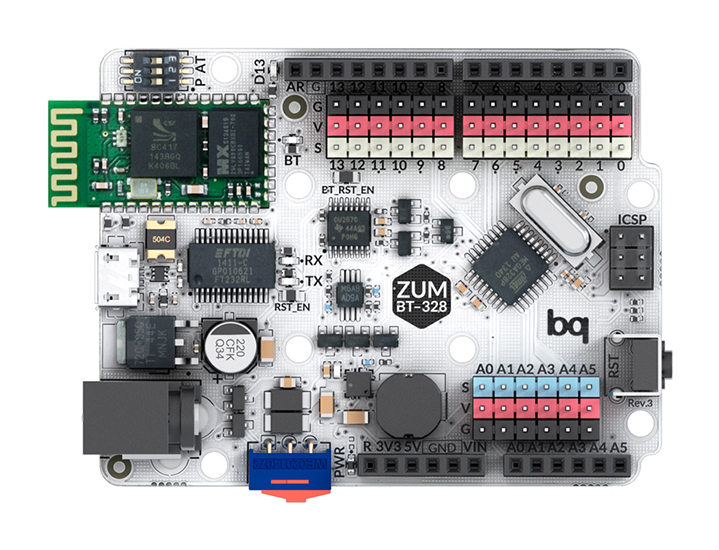
\includegraphics[width=0.6\textwidth]{Figures/BQZUM}
\caption[BQ Zum Bluetooth empleada para mover los servos]{BQ Zum Bluetooth empleada para mover los servos}
\label{fig:BQZUM}
\end{figure}


%-----------------------------------
%	SUBSECTION 1: VISIÓN
%-----------------------------------
\subsection{Cámara visión por computador}

Se realiza una prueba piloto aprovechando el sistema de visión instalado para otro proyecto, compuesto por la cámara fija de Fanuc, 2 paneles LED de luz difusa (60W) y el software de visión Fanuc: iRvision. Se elige realizar las pruebas en ésta plataforma, y no en un ordenador convencional con matlab u opencv, por inmediatez, el sistema está ya calibrado y en funcionamiento, además de que cuenta con un rack de salidas y entradas digitales; como se ha dicho, el objetivo era comprobar la viabilidad.

El sistema de visión está conectado al controlador de un brazo robótico LRMate 200iD, con un módulo I/O digitales a 24 voltios. Por lo que se realiza una interfaz con 2 relés para comunicar con la placa Arduino (5V), encargada de calibrar los servos del juguete.

En la figura \ref{fig:CeldaFanuc} podemos ver el área de trabajo de la celda robótica y su cámara.

\begin{figure}
\centering
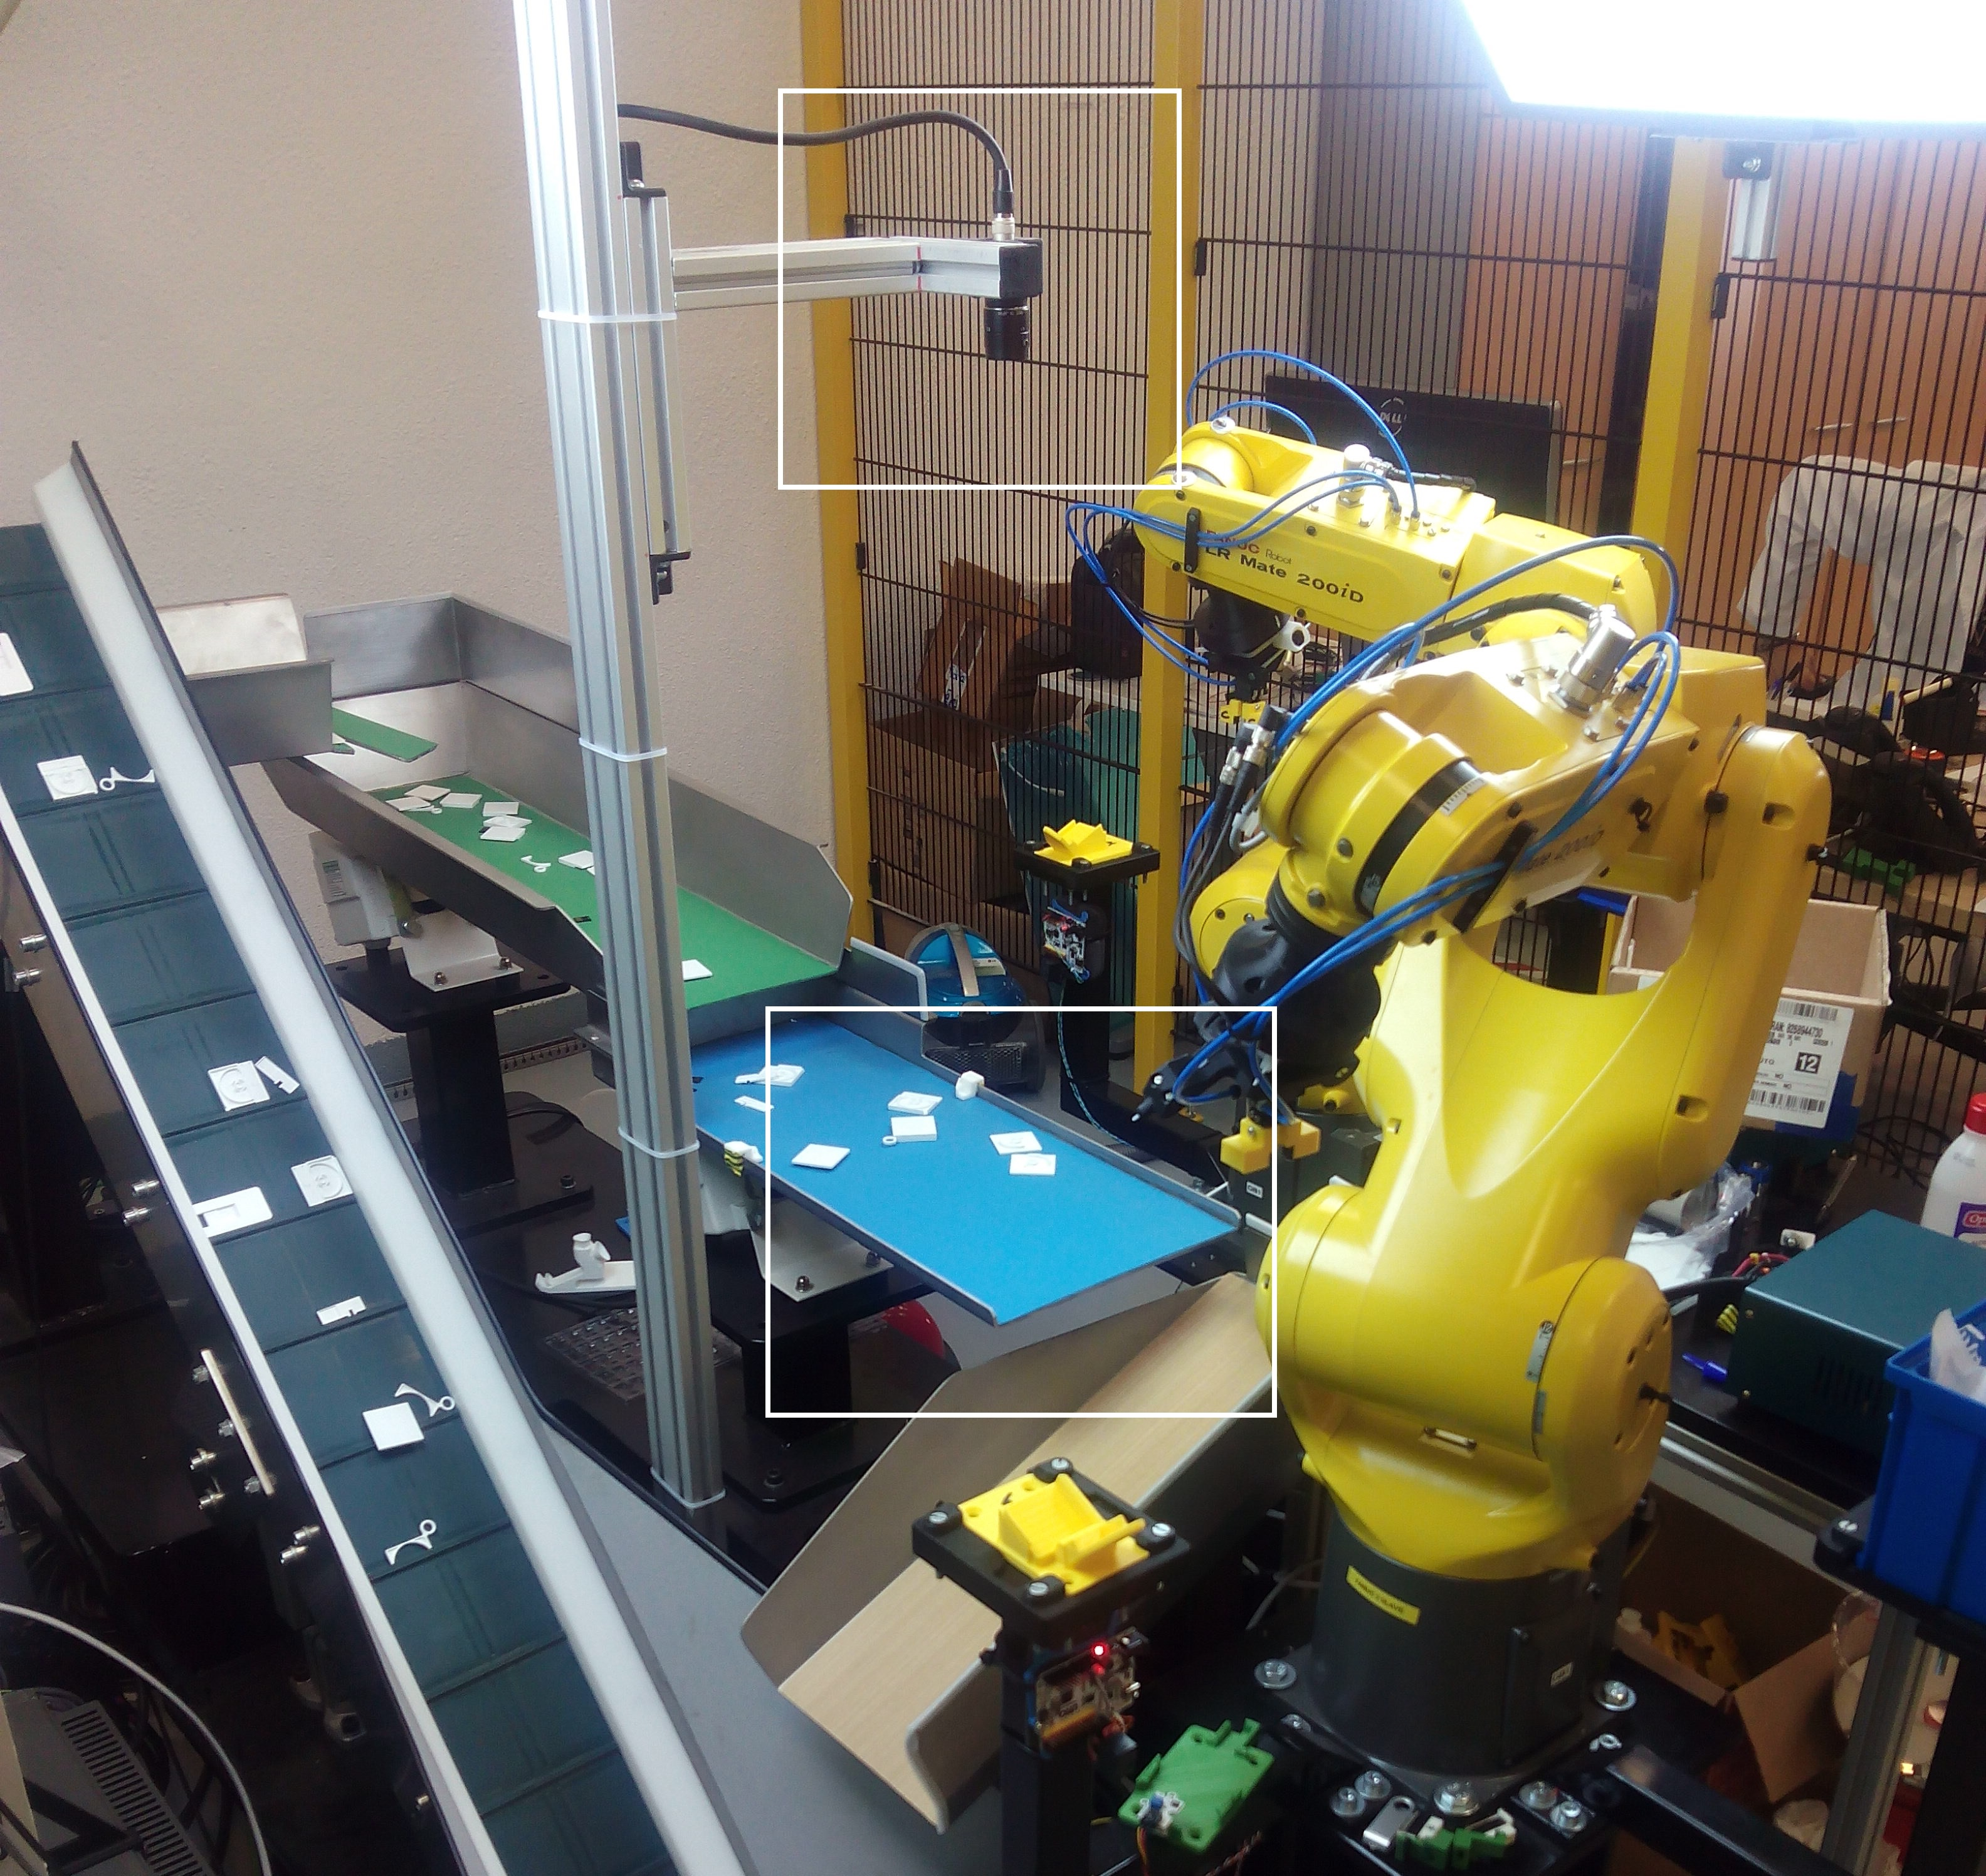
\includegraphics[width=120mm]{Figures/CeldaFanuc}
\caption[Celda con cámara de Fanuc]{Celda con cámara de Fanuc}
\label{fig:CeldaFanuc}
\end{figure}

El programa creado en Arduino recibe como entradas dos señales que indican en qué sentido se debe girar el servo. Como salida, actúan sobre el servo hacíendolo corregir su posición iterativamente 1 grado cada segundo hasta alcanzar la posición deseada.

La posición deseada es definida utilizando iRvision (Software de visión de Fanuc), mediante técnicas de visión por computador (Localización de elementos entrenados, medición de distancias y ángulos entre ellos). Para el caso del "tobillo", buscando perpendicularidad con la "cadera", y para ésta, consiguiendo cierta distancia entre dos líneas paralelas. Se pueden ver las Figuras \ref{fig:Tobillo} y \ref{fig:Cadera}.

\begin{figure}
\centering
\begin{minipage}{.5\textwidth}
  \centering
  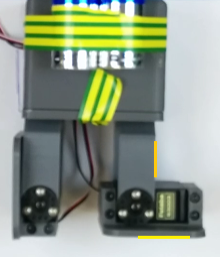
\includegraphics[width=.7\textwidth]{Figures/Tobillo}
  \captionof{figure}{Calibración tobillo con visión}
  \label{fig:Tobillo}
\end{minipage}%
\begin{minipage}{.5\textwidth}
  \centering
  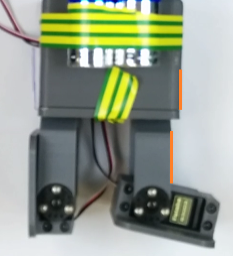
\includegraphics[width=.7\textwidth]{Figures/Cadera}
  \captionof{figure}{Calibración cadera con visión}
  \label{fig:Cadera}
\end{minipage}
\end{figure}


%-----------------------------------
%	SUBSECTION 2: IMUS
%-----------------------------------

\subsection{Sensores IMUs}
Para la segunda prueba se emplea una placa que combina un giróscopo, acelerómetro y magnetómetro para formar una unidad de medición inercial (de ahora en adelante IMU) con una precisión de hasta 0.1 grados.

\subsubsection{Teoría}

La MinIMU-9 v3 (Figura \ref{fig:MinIMU_board} fue seleccionada de entre varias opciones, como la famosa MPU6050, la GY-87 o la versión v2 de MinIMU (todas de un precio similar), por la precisión y repetibilidad de las lecturas, además de parecer un dispositivo ampliamente utilizado y probado por la comunidad.

\begin{figure}
\centering
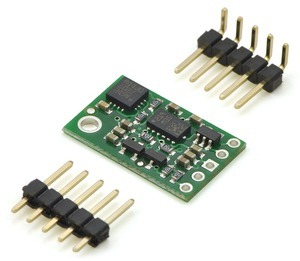
\includegraphics[width=65mm]{Figures/MinIMU_board}
\caption[MinIMU-9 v3 de Pololu]{MinIMU-9 v3 de Pololu}
\label{fig:MinIMU_board}
\end{figure}

Tras estudiar el comportamiento del sensor, y una fase de documentación acerca de las opciones de que se dispone, surgen tres posibilidades:

\begin{itemize}
  \item Librería de Pololu "MinIMU-9 AHRS"
  \item Librería "Open IMU"
  \item Desarrollar la matemática tomando los valores RAW del sensor
\end{itemize}

A pesar de lo atractivo de la tercera opción, no se disponía de suficiente tiempo para seguir adelante con ella, se trató de comprender el funcionamiento de las 2 librerías ya creadas.

Por simplicidad, Open IMU resultaba llamativa, pero rápidamente se percibió que podía quedarse demasiado corta y que las lecturas obtenidas empleando ésta librería (los ángulos euler de pitch, roll y yaw) parecían no tener la repetibilidad necesaria para nuestra aplicación, por otro lado, hacía más de 3 años que no se realizaban cambios en su repositorio GIT, por lo que posiblemente estaba preparada para funcionar con la versión anterior de la placa, MinIMU-9 v2, con una exactitud de hasta 1 grado solamente.

La línea elegida fue la de la librería recomendada por Pololu (fabricante del dispositivo), dejando un poco limitado el modo de funcionar pero ofreciendo un acceso rápido a las mediciones del sensor en forma de posición en ángulos euler.

Para un correcto funcionamiento del magnetómetro, se han de configurar los valores máximos y mínimos de las lecturas del acelerómetro, estos 2 sensores se encuentran en el encapsulado LSM303, la librería de dicho chip proporciona un programa de Arduino que captura dichas mediciones y salva la mayor mientras movemos la placa en todas las orientaciones posibles, mostrandola por el puerto serie. Los valores obtenidos se han de escribir, sustituyendo los "por defecto", en la cabecera de la misma librería.

La limitación de ésta librería que se había comentado antes , es que para obtener con precisión los ángulos euler en todas las orientaciones, se debe llamar una función de la librería \textbf{calibrateIMU()} con la placa colocada en una de las 2 posiciones que se ven en la Figura \ref{fig:IMU_positions}, lo más paralelo al suelo posible, con ésta función definimos en el espacio el 0 de los ejes X e Y del sistema, por lo que se corrigen desvíos si la posición no es totalmente horizontal, sin embargo, ésto deriva en errores que crecen en proporción a la inclinación que se de en alguno de los ejes. Se elige una de ellas configurando ciertos parámetros de la librería de Pololu en el programa principal.

\begin{figure}
\centering
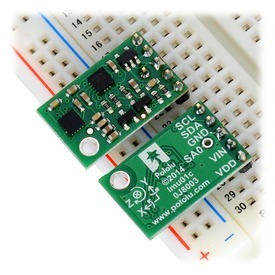
\includegraphics[width=65mm]{Figures/IMU_positions}
\caption[Posiciones calibración IMU]{Posiciones calibración IMU}
\label{fig:IMU_positions}
\end{figure}

La orientación en Z depende de la brújula y su tiempo de estabilización es lento, por ello, se piensa en emplear los giros en los otros 2 ejes, X e Y, por lo que la posición del robot ha de ser la de acostado sobre un lado, descartando las posiciones que, de entrada, parecen más razonables como boca arriba/boca abajo, o con las piernas hacia arriba. Ver Figuras \ref{fig:patas_arriba} y \ref{fig:acostado}.

\begin{figure}
\centering
\begin{minipage}{.5\textwidth}
  \centering
  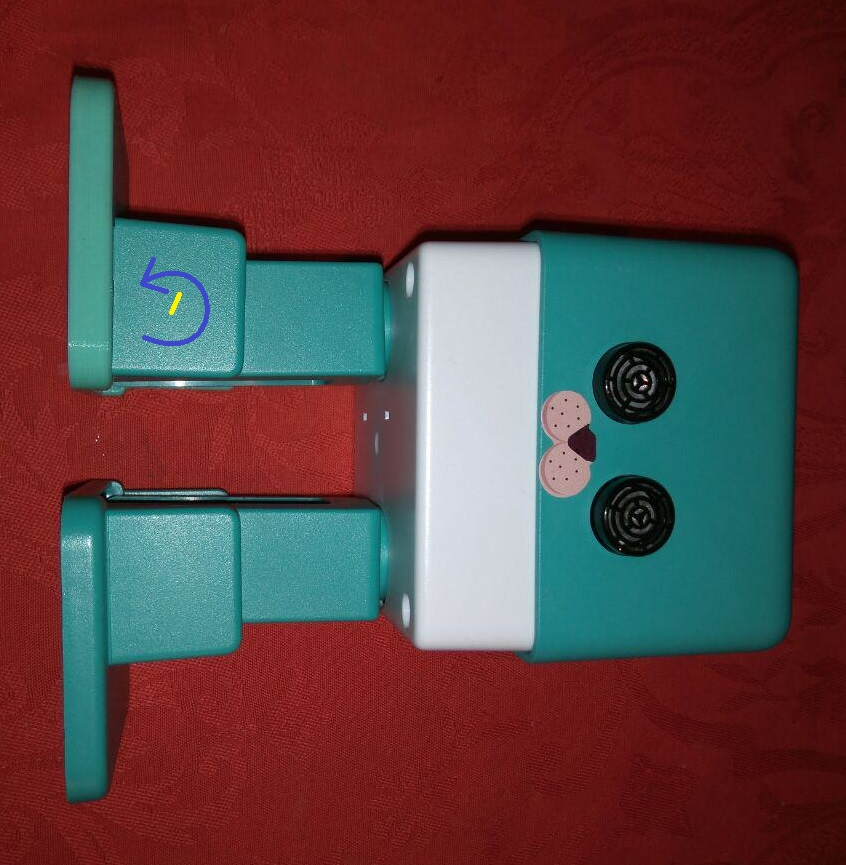
\includegraphics[width=.9\textwidth]{Figures/acostado}
  \captionof{figure}{Tobillo gira sobre eje Z}
  \label{fig:acostado}
\end{minipage}%
\begin{minipage}{.5\textwidth}
  \centering
  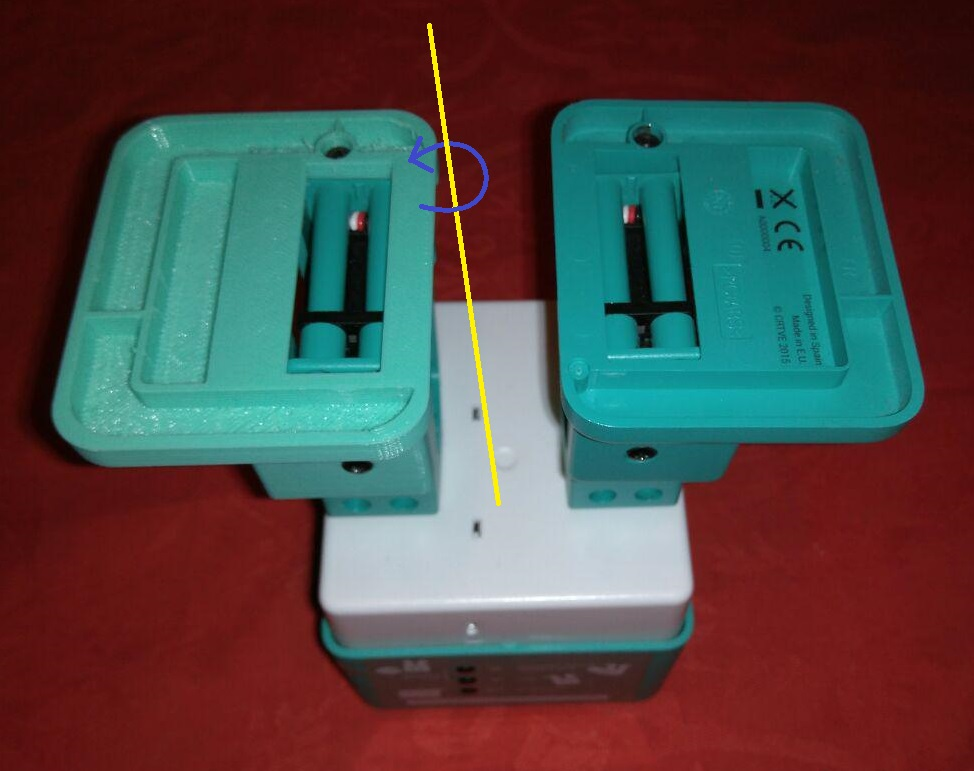
\includegraphics[width=.9\textwidth]{Figures/patas_arriba}
  \captionof{figure}{Cadera gira sobre eje Z}
  \label{fig:patas_arriba}
\end{minipage}
\end{figure}


\subsubsection{Prueba inicial}

Se programa el algoritmo empleando una máquina de estados en la misma placa controladora de Zowi con un pulsador para pasar de un estado a otro. Versión muy básica para probar el concepto. Se emplea comunicación serie para conocer el estado del sensor y una grapa impresa para acoplarlo al pié del Zowi.

El procedimiento programado sería:
\begin{itemize}
  \item Iniciar el sistema -- Automáticamente se produce la calibración de la IMU
  \item Colocar el sensor en el pié de Zowi
  \item Pulsar el botón -- Se inicia la calibración del servo
\end{itemize}

El modo de calibración del servo consiste en dar un primer valor a la posición que debería tener el servo, es decir, 0º para la cadera o 90º para el pie, entonces se lee el sensor para ver el error cometido y se ajusta la posición del servo teniendo en cuenta la diferencia del valor deseado y la nueva lectura, se repite hasta 2 veces.

Se obtienen buenas sensaciones con éste método y se nota de inmediato que el éxito del mismo radica en la correcta calibración inicial del sensor y en una buena fijación al pié del robot, por lo que se desarrolla un zapato para montar en él el sensor y un soporte para el robot, junto a otro soporte para realizar la calibración del sensor (ya integrado en el zapato) en la misma pieza. De esta forma se garantiza la correspondencia y paralelismo de los planos de apoyo de ambas partes (robot – zapato).

%-----------------------------------
%	Conclusiones
%-----------------------------------

\subsection{Conclusiones}
El método de calibración empleando visión muestra buenos resultados y es muy mejorable si se emplea software creado específicamente para la aplicación, sin embargo, las condiciones de iluminación y posición han de ser las mismas o muy parecidas para cada banco de trabajo para garantizar un buen funcionamiento del software, por lo que su instalación, puesta en marcha y configuración, son delicados y se deberían hacer in-situ. En el momento de las pruebas de validación aún se desconoce la ubicación de la fábrica y la nave de montaje -posiblemente en China o Polonia-,  la solución se encarece considerablemente si se han de realizar desplazamientos para llevar a cabo la instalación y puesta en marcha.

Con las IMUs se obtuvieron buenos resultados y se tenía bastante claro que se quería seguir adelante con ellas por su bajo coste y y su fácil implementación. Quedaba afinar el algoritmo de calibración implementando una máquina de estados mucho más robusta y endureciendo el criterio de validación automática de una buena calibración para obtener mejores resultados. En el siguiente subcapítulo se desarrolla su evolución.

%----------------------------------------------------------------------------------------
%	SECTION 3: Laboratorio
%----------------------------------------------------------------------------------------

\section{Prototipo de laboratorio}

Se decide continuar con la solución de las IMUs y se producen reuniones cada pocos días/semanas entre los diferentes grupos implicados en el desarrollo del juguete Zowi (mecánica, hardware, producto, automatización...) dónde las especificaciones el banco de calibración van tomando forma en función de los resultados obtenidos. En la presente sección se mostrará la línea de evolución del prototipo, mencionando las características y mejoras más relevantes añadidas, así como las pruebas realizadas antes de pasar al desarrollo de la versión final.

\subsection{Línea de evolución}

Tras elegir la línea de los sensores IMU, se comienza a trabajar de inmediato en la mejora de la solución.

\subsubsection{Primeras mejoras}

La máquina de estados es mejorada, diferenciando calibraciones malas de calibraciones buenas. Se añaden una indicador led y uno acústico para resaltar el resultado con diferentes sonidos. Esta mejora se mantendrá hasta la versión final del producto.

La siguiente necesidad a cubrir sería garantizar que el robot comparte el plano con el sensor, que ha de ser calibrado antes de colocarse en el robot como explicamos en la sección anterior. Hasta ahora el sensor era fijado utilizando una grapa impresa (Ver Figura \ref{fig:grapa}).
Se monta el sensor en una pieza especialmente diseñada e impresa para colocarla en el pié de Zowi, razón por la que es llamada "Zapato".
Se crea también una base donde se coloca el Zowi, con un área para colocar el zapato en el momento de su inicialización, dónde el sensor es calibrado. Se puede ver el banco en la Figura \ref{fig:banco_1zapato}.


\begin{figure}
\centering
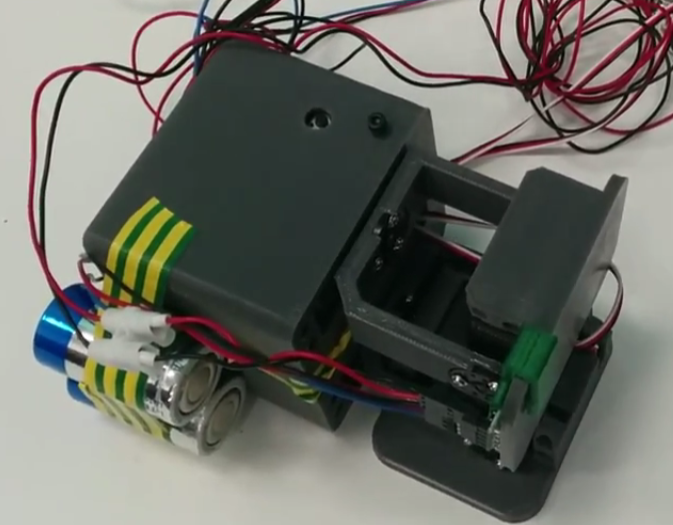
\includegraphics[width=70mm]{Figures/grapa}
\caption[Sensor anclado con grapa impresa]{Sensor anclado con grapa impresa}
\label{fig:grapa}
\end{figure}


\begin{figure}
\centering
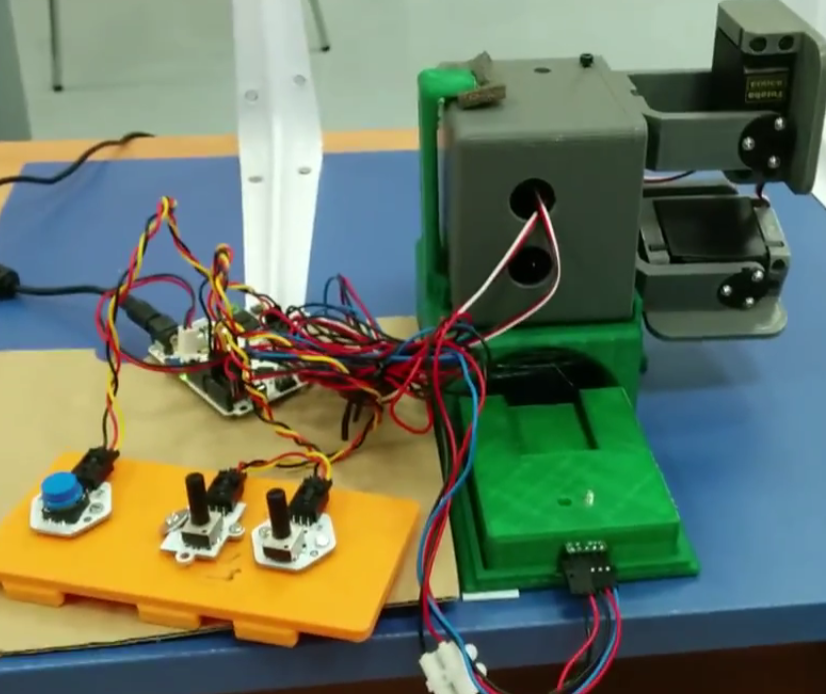
\includegraphics[width=80mm]{Figures/banco_1zapato}
\caption[Bancos impresos para Zowi y zapato]{Bancos impresos para Zowi y zapato}
\label{fig:banco_1zapato}
\end{figure}

El algoritmo hasta ahora pasaba por calibrar una pierna del juguete solamente, haciendo ambas partes -tobillo y cadera-. Se mejora este punto, conectando a la placa controladora 2 sensores IMUs. La comunicación con la MinIMU-9 se realiza a través de I\textsuperscript{2}C, y su interfaz permite seleccionar facilmente entre 2 direcciones distintas para el giróscopo, y lo mismo para el acelerómetro/brújula. Para ello solamente tenemos que conectar SA0 a GND. (Ver Figura \ref{fig:minimu_sa0} y Tabla \ref{tab:IMU-I2C})

\begin{table}
\centering
\begin{tabular}{l c c}
\toprule
\tabhead{Sensor} & \tabhead{Slave Add. - default} & \tabhead{Slave Add. - SA0 driven low} \\
\midrule
L3GD20H (gyro) & 1101011b & 1101010b \\
LSM303D (acc+magnet) & 0011101b & 0011110b \\
\bottomrule\\
\end{tabular}
\caption{Direcciones de esclavo I\textsuperscript{2}C para MinIMU-9 v3}
\label{tab:IMU-I2C}
\end{table}

\begin{figure}
\centering
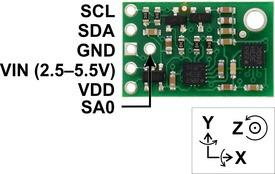
\includegraphics[width=60mm]{Figures/minimu_sa0}
\caption[MinIMU-9 v3 Pin-out]{MinIMU-9 v3 Pin-out}
\label{fig:minimu_sa0}
\end{figure}

Es necesario cambiar las direcciones de una de las placas, de lo contrario ambas tendrían las mismas direcciones de esclavo I\textsuperscript{2}C y causaría un mal funcionamiento el intentar leer de una de ellas. Además, se mejora el banco impreso para poder albergar los 2 zapatos y la máquina de estados, implementando la calibración de ambas piernas y aumentando número de iteraciones e incluyendo un filtrado de múltiples medidas para evitar leer ruido. Ver Figura \ref{fig:banco_2zapato}.

\begin{figure}
\centering
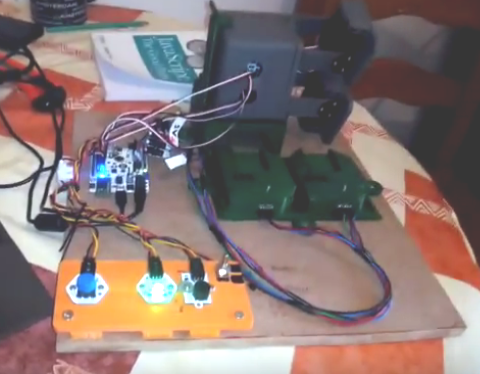
\includegraphics[width=70mm]{Figures/banco_2zapato}
\caption[Banco 1 zapato]{Banco impreso para Zowi y 2 zapatos}
\label{fig:banco_2zapato}
\end{figure}

La calibración/inicialización de los sensores muestra resultados, como se ha comentado anteriormente, no tan buenos cuando el sensor se inclina notablemente. Por ello que el éxito de la calibración de la cadera (0º de set point) es mayor que el de la calibración del pié (90º). Se considera corregir el set point de los piés en la fase de calibración de los sensores.

Se diseñan unos cajetines para el ajuste del sensor a los 90º, de modo que antes de comenzar la calibración de los juguetes, el sensor (zapato), debe ser calibrado en las posiciones horizontal y vertical.

Se impide avanzar en el procedimiento si tras calibrar los sensores al inicio, las medidas obtenidas difieren demasiado de 0º en ambos ejes, se vuelve a un estado en el que se espera pulsar el botón para volver a realizar la calibración, es decir, se comienza a implementar una gestión de errores.

Se añaden al conjunto un nivel y unos tornillos para regular la inclincación y mantener todo lo más horizontal posible antes de comenzar. Ver Figura \ref{fig:banconivel}.

\begin{figure}
\centering
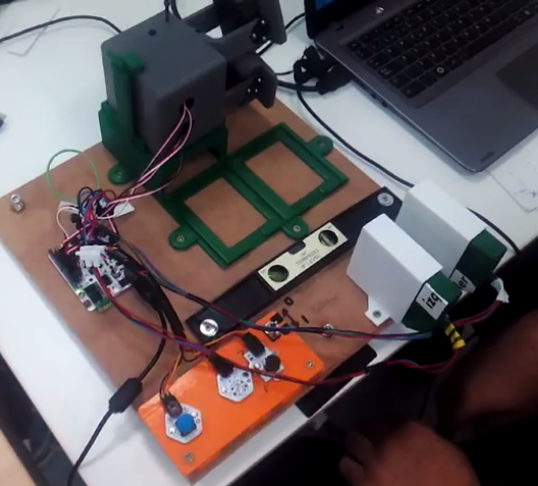
\includegraphics[width=80mm]{Figures/banco_nivel}
\caption[Banco con inclinación regulable]{Banco con inclinación regulable}
\label{fig:banconivel}
\end{figure}

%-----------------------------------
%	SUBSUBSECTION 1
%-----------------------------------
\subsubsection{Tomando forma}

Hasta ahora todas las pruebas se habían realizado en la misma controladora de Zowi. Se recibe información sobre la placa que será empleada para los robots (en desarrollo por el Dpto. de Hardware), se conoce que el número de entradas/salidas será reducido y ajustado a los sensores/actuadores del propio juguete, por lo que realizar todas las conexiones que planteamos en nuestras pruebas en la misma placa junto a todos los periféricos de zowi no es una opción.

Se plantea el uso de otra placa conectada por I\textsuperscript{2}C a la placa controladora del Zowi (por ahora una ZUM BT) y la librería Wire.h de Arduino. Zum BT es una versión de la Arduino UNO con bluetooth incorporado, y una etapa de potencia capaz de sacar hasta 3.2 amperios por sus salidas digitales.

La nueva placa empleada sería una Freeduino Mega, versión basada en la Mega, es elegida por ser compatible con todo lo desarrollado y por su bajo coste para la empresa y por presentar una cantidad de entradas y salidas mayor que los modelos UNO.

Se vuelven a diseñar unos bancos para calibrar los sensores tanto horizontal como verticalmente, es decir, inicializar ejes y ajustar el eje Y en vertical. Todo en el mismo espacio, como se puede ver en la Figura \ref{fig:bancov3}.

\begin{figure}
\centering
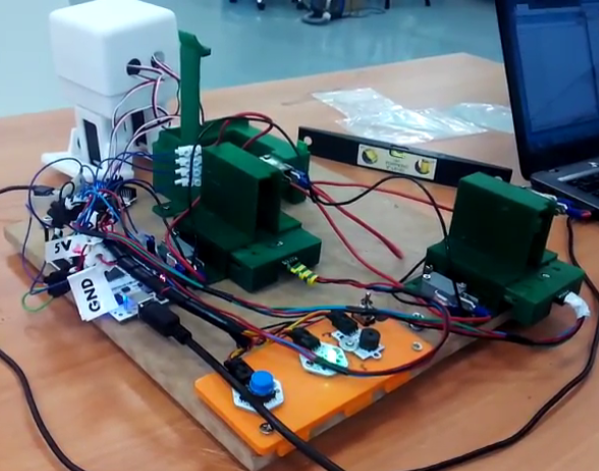
\includegraphics[width=110mm]{Figures/banco_v3}
\caption[Banco con conexión MEGA-ZUM]{Banco con conexión MEGA-ZUM}
\label{fig:bancov3}
\end{figure}

El empleo de una Mega nos proporciona una gran cantidad de pines de entrada salida, se incorporan al sistema unos finales de carrera para detectar que los zapatos están en la posición correcta para su calibración.

Como característica \textbf{principal}, se diseña una interfaz de comunicación entre ambas placas mediante I\textsuperscript{2}C, se construyen determinadas "instrucciones" en la placa Mega (placa con la máquina de estados) y un programa que funciona como intérprete que es cargado en la ZUM (placa del robot), se encarga de traducir las instrucciones recibidas de la otra placa por I\textsuperscript{2}C en movimientos de servos, entre otras cosas. Puede verse la arquitectura del sistema en la Figura \ref{fig:v3-diag}.

\begin{figure}
\centering
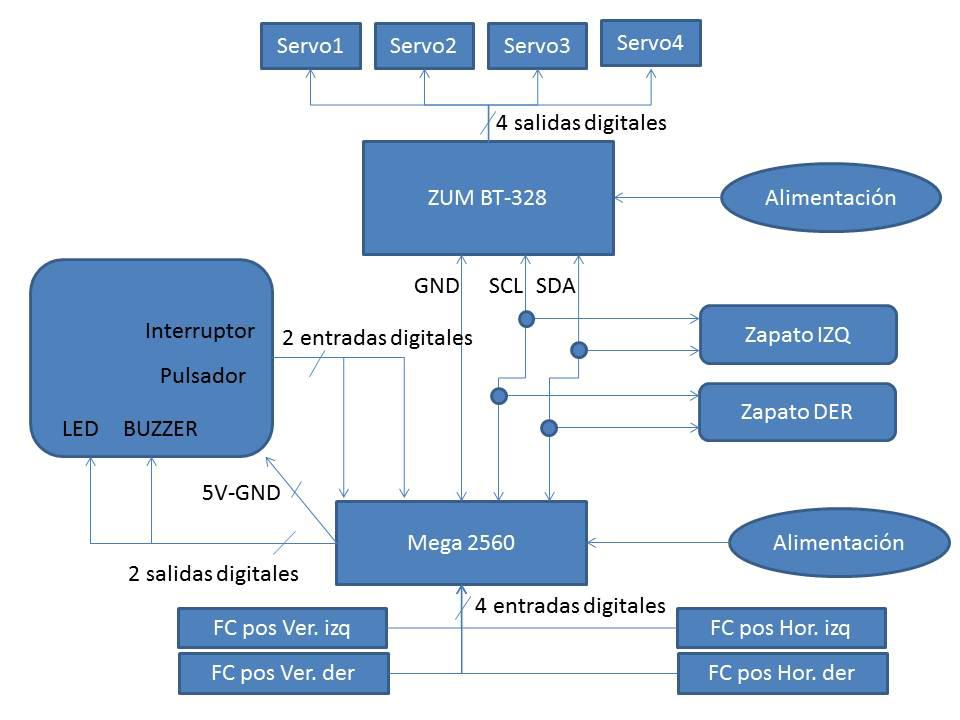
\includegraphics[width=120mm]{Figures/v3-diag}
\caption[Arquitectura versión MEGA-ZUM por I\textsuperscript{2}C]{Arquitectura versión MEGA-ZUM por I\textsuperscript{2}C}
\label{fig:v3-diag}
\end{figure}

La máquina de estados se hace más robusta en general, detectando fallos y facilitando la recuperación para un correcto funcionamiento.

Al final de esta etapa se conoce la controladora que llevará el juguete, así como la versión -prototipo- de Zowi definitiva, sinterizada por láser, en lugar de inyectada, pero ya con sus dimensiones y forma finales. Se puede ver en la Figura \ref{fig:zowi-sls}.

\begin{figure}
\centering
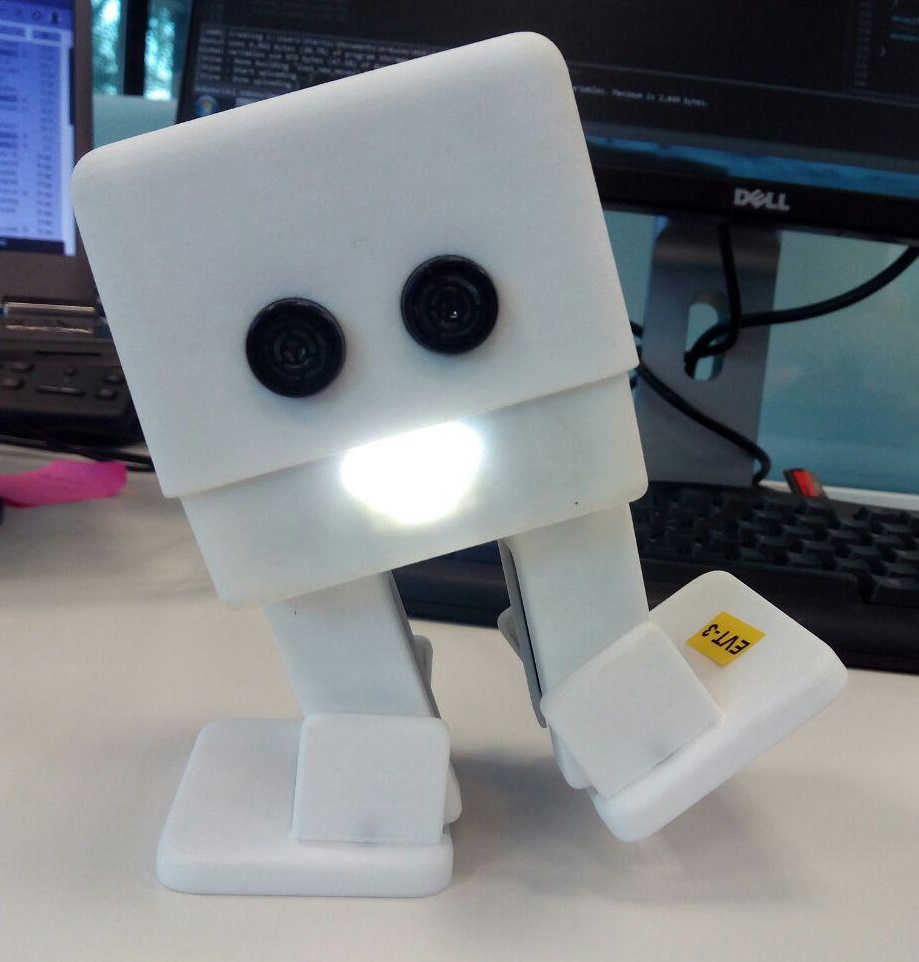
\includegraphics[width=70mm]{Figures/zowi-sls}
\caption[Prototipo final Zowi SLS]{Prototipo final Zowi SLS}
\label{fig:zowi-sls}
\end{figure}

\subsubsection{Prototipo final: Banco de Calibración}

En este punto se produce el mayor cambio en el proyecto. La solución de comunicación por I\textsuperscript{2}C entre las diferentes placas asumía que la controladora de Zowi tendría accesibles los pines al micro para I\textsuperscript{2}C y SPI (cosa incierta) y, además, hacía necesario el acceso al interior del robot, que en principio, podría llegar ya montado de las etapas de producción anteriores. Se sugiere implementar la comunicación a través del puerto USB que tendrá la placa de Zowi.

Las controladoras Arduino pueden ser esclavos serie por USB, no maestros, realizar una comunicación serie de una a otra no es posible, de ahí que se plantee usar una Raspberry PI (Figura \ref{fig:raspi}) como maestro Serie de ambas placas, esclavos serie, sustituyendo la interfaz I\textsuperscript{2}C implementada en la versión anterior y haciendo de puente entre ambas.

Se contempló la posibilidad de quitar la Mega y emplear solamente la Raspberry como núcleo del sistema, sin embargo, eso conllevaría rehacer gran parte del trabajo y encontrar la forma de hacer funcionar los sensores con éste dispositivo, lo que requería un tiempo que no se tenía.

Una primera iteración fue la de sustituir la comunicación por I\textsuperscript{2}C, por la comunicación serie, se adaptaron los programas de MEGA y de ZUM. La comunicación era unidireccional. Mega > Raspberry > Zowi. La Raspberry PI funcionaba como mero driver de comunicaciones:
\begin{itemize}
  \item Se modificaron los comandos enviados con la librería Wire.h desde la freeduino Mega para ser comandos enviados por serie (Librería Serial.h) con ciertos caracteres de inicio y fin de comunicación a modo de protocolo (desarrollado específicamente para esta aplicación).
  \item Se implementó en la Raspberry un programa en Python que hacía de intérprete. Haciendo escucha a la comunicación serie abierta con la Freeduino Mega, y enviando comandos a la placa controladora de Zowi a través de la comunicación Serie abierta con ella.
\end{itemize}

La incorporación al sistema de una Raspberry PI, un ordenador al fin y al cabo, abría gran cantidad de mejoras de fácil implementación, por lo que se aprovechó la ocasión para desarrollar un prototipo "casi definitivo", no solamente a nivel de software.

Se decide introducir la electrónica en un armario eléctrico y, a su vez, emplear el mismo como estructura del soporte de Zowi y de los zapatos. Ver Figura \ref{fig:bancov4}. Se integran nivel y patas regulables.

\begin{figure}
\centering
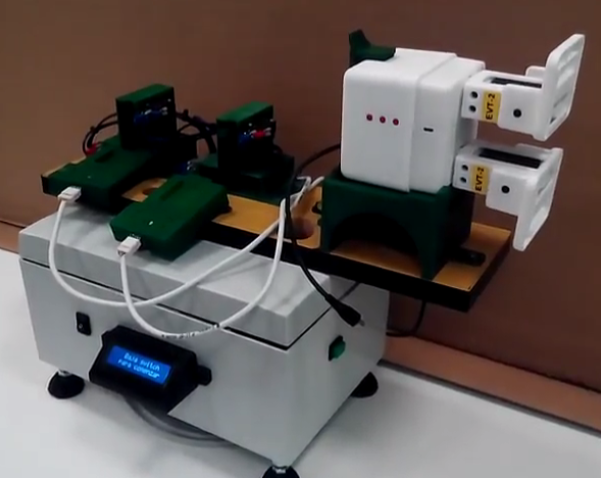
\includegraphics[width=110mm]{Figures/banco_v4}
\caption{Banco prototipo final}
\label{fig:bancov4}
\end{figure}

Se introdujo un display LCD conectado a la Mega por I\textsuperscript{2}C que hacía más fácil la interacción del usuario con el banco de calibración y se trabajó en mejorar la máquina de estados para hacer el uso del sistema más amigable; y se mejoró el conexionado añadiendo una PCB custom como shield de la Mega, que ofrecía borneros para conectar los leds, display LCD, IMUs, finales de carrera y botones.

Durante el proceso de calibración se guardarán los offsets calculados en ciertas posiciones de la memoria EEPROM de la placa controladora de Zowi. Se usa para ello la librería EEPROM.h. Esto es necesario para el funcionamiento de los programas por defecto, cuyas librerías (zowi.h y oscillator.h) están configuradas para usar los valores en dichas posiciones de la memoria.

Multitud de mejoras software definitivas fueron implementadas en esta fase para aumentar su funcionalidad, en el subcapítulo siguiente se verán en mayor detalle, a destacar:
\begin{itemize}
  \item Raspberry utilizada como programador, empleando la utilidad AVRDUDE cargará el programa de calibración en cada Zowi.
  \item Cargará, del mismo modo y al finalizar la calibración, el programa de fábrica con que saldrá a la venta el producto. Sobrescribiendo el de calibración.
  \item Se le habilita acceso remoto por SSH y por XRDP para poder acceder a ella desde fuera.
  \item Se instala un servidor de MySQL y se configura para guardar datos tanto en local como en nuestros servidores.
  \item El entorno de programación de Arduino es instalado, para poder modificar la Mega directamente desde Raspberry.
\end{itemize}

%-----------------------------------
%	SUBSECTION 2
%-----------------------------------

\subsection{Pruebas realizadas}


Durante todo el desarrollo se han realizado pruebas, sin embargo, se comentan los resultados la prueba previa a MP (massive production), realizada con el prototipo final. La Figura \ref{fig:pre-mp} muestra el armario de calibración preparado para la prueba.

Los operadores fueron compañeros que no habían tenido contacto alguno con la máquina, haciendo de operarios de forma distraída.
\begin{figure}
\centering
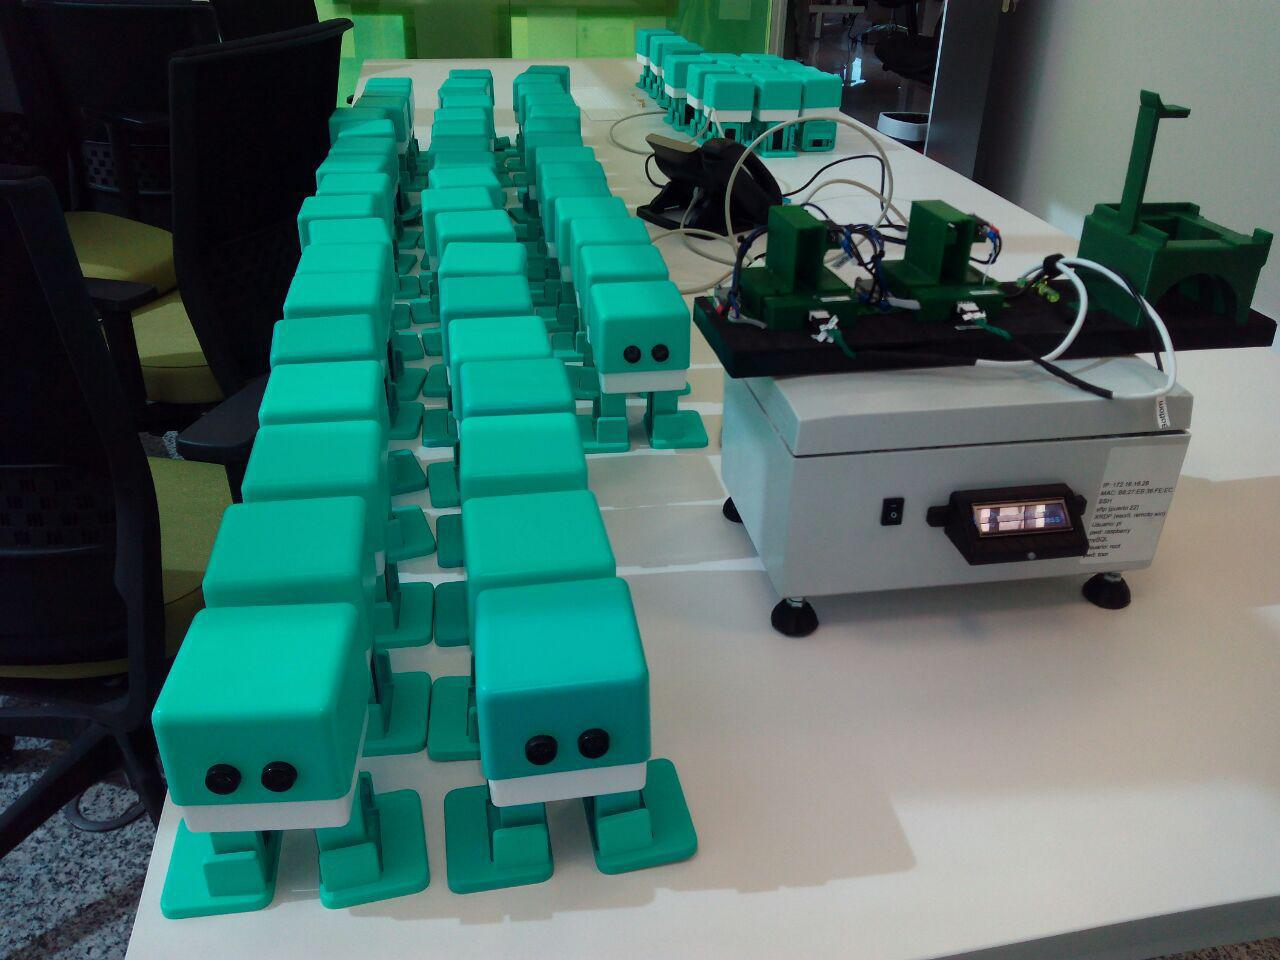
\includegraphics[width=110mm]{Figures/pre-mp}
\caption{Prueba pre MP}
\label{fig:pre-mp}
\end{figure}

Se logran calibrar satisfactoriamente 62 juguetes, con solamente 1 contratiempo: Al no respetar el protocolo en cuanto a órden de operaciones, concretamente, intento de programar la placa sin energizar. Si se intenta programar la placa conectada pero sin encender, el programador AVRDude realiza hasta 10 intentos de programarla sin éxito; al energizarla durante los intentos, según en qué momento se haga, puede ser recuperable, o puede llevar al sistema a un estado de fallo. Se tuvo que reiniciar y volver a hacer la calibración de los zapatos. A pesar de ser un error de operador, se intenta corregir para la versión final.

Un total de 4 veces se produce una calibración mala, inducidas para poner a prueba el sistema, el sistema notifica (Display y sonido) la calibración como mala y se necesita que se vuelva a pulsar el botón. De ahí una calibración de apenas unos segundos en las gráficas siguientes, por no tener que conectar y calzar al juguete).

Analizando la información extraída de la base de datos tras las calibraciones, se muestra (Figura \ref{fig:tiempos}) Segundos vs. n\textsuperscript{o} Zowi, una segunda gráfica (Figura \ref{fig:ok-nok}) muestra 1 para calibraciones válidas, 0 para las declaradas fallidas. Los tiempos del primer y último registro no son representativos.

\begin{figure}
\centering
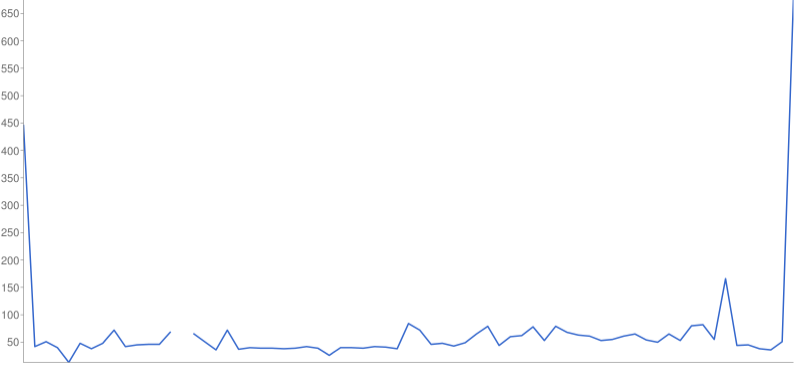
\includegraphics[width=140mm]{Figures/tiempos}
\caption{Segundos por cada calibración de Zowi}
\label{fig:tiempos}
\end{figure}

\begin{figure}
\centering
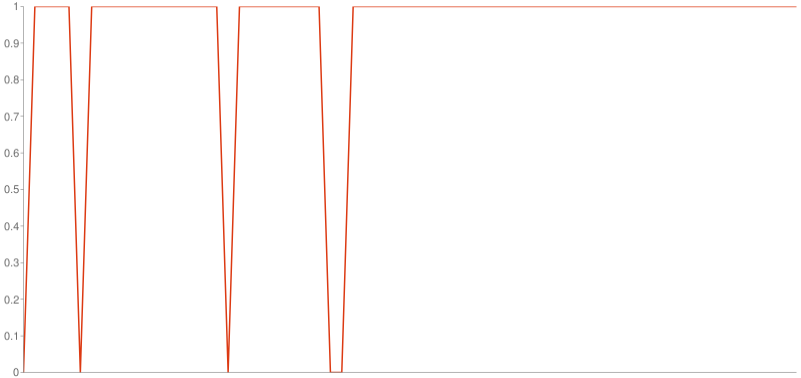
\includegraphics[width=140mm]{Figures/ok-nok}
\caption{OK:1 | NOK:0 - para cada calibración de Zowi}
\label{fig:ok-nok}
\end{figure}

%----------------------------------------------------------------------------------------
%	SECTION 4: Finales
%----------------------------------------------------------------------------------------

\section{Armarios finales}

El trabajo asignado al autor del proyecto debió haber concluido con el prototipo presentado en el subcapítulo anterior, dejando por diseñar una versión definitiva de los soportes y zapatos del banco al Dpto. de Mecánica de BQ, y el montaje de tantos armarios y bancos como fuese necesario para abordar la producción de todos los juguetes a Rosti (empresa de extrusión de plásticos y montaje subcontratada en Polonia), encargados del ensamblado de los robots Zowi; sin embargo, se decidió realizar el montaje de 2 armarios con ligeras modificaciones y planos eléctricos para enviar a Polonia ya probados y validados. Ver armarios en Figura \ref{fig:armariosFinales}.

\begin{figure}
\centering
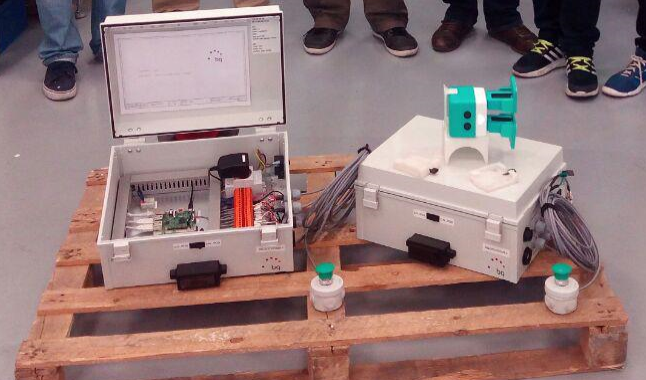
\includegraphics[width=110mm]{Figures/armariosFinales}
\caption{Armarios finales preparados para su envío a fábrica}
\label{fig:armariosFinales}
\end{figure}

Modificaciones destacables respecto al prototipo:
\begin{itemize}
  \item Armario de componentes eléctricos separado de la parte mecánica, se siguieron utilizando los diseños impresos de versiones anteriores para validación del funcionamiento, pero las piezas finales quedaban a cargo del Dpto. de Mecánica. Éste nuevo armario sería más amplio que el anterior.
  \item Mangueras de cables más largas (pues armario y banco de calibración irán separados).
  \item Pulsador exterior con una manguera de cable para ser colocado donde se desee en fábrica, en lugar del pulsador en el lateral del armario de la versión anterior.
  \item Conexión USB y Ethernet por pasamuros al interior del armario.
  \item Cambios en el diseño del cajetín del display LCD, pues el armario irá colocado a la altura de los ojos del operador.
\end{itemize}

%-----------------------------------
%	SUBSECTION 1
%-----------------------------------
\subsection{Componentes e implementación física}

\subsubsection{Arquitectura y conexiones}

El diagrama que se puede ver en la Figura \ref{fig:diagFinal}, muestra, a grandes rasgos, un esquema de las conexiones entre los principales dispositivos que intervienen en el sistema. El sistema completo consta del armario eléctrico, además del juguete Zowi conectado al armario. Por ello se muestran en el esquema tanto las placas internas del armario (Mega y Raspberry), como la placa controladora de Zowi (Zum).

\begin{figure}
\centering
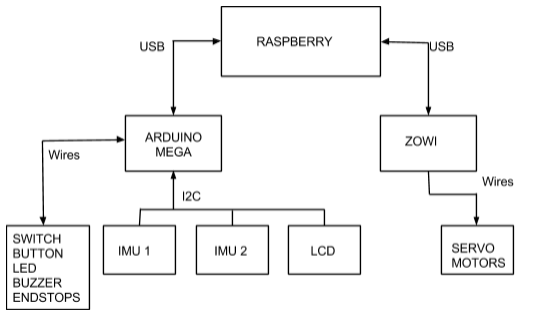
\includegraphics[width=100mm]{Figures/diagFinal}
\caption{Esquema de conexiones}
\label{fig:diagFinal}
\end{figure}

\subsubsection{Armario eléctrico}

Se elige instalar la parte fija del sistema en una placa de montaje dentro de un armario eléctrico de 40x30x18cm. Se emplean canaletas y bornas en un carril DIM para facilitar las conexiones al exterior del armario. Se utilizan pasamuros para las mangueras a pulsador y sensores IMU, así como para conexión USB (Raspberry - Zowi) y RJ45.

\begin{figure}
\centering
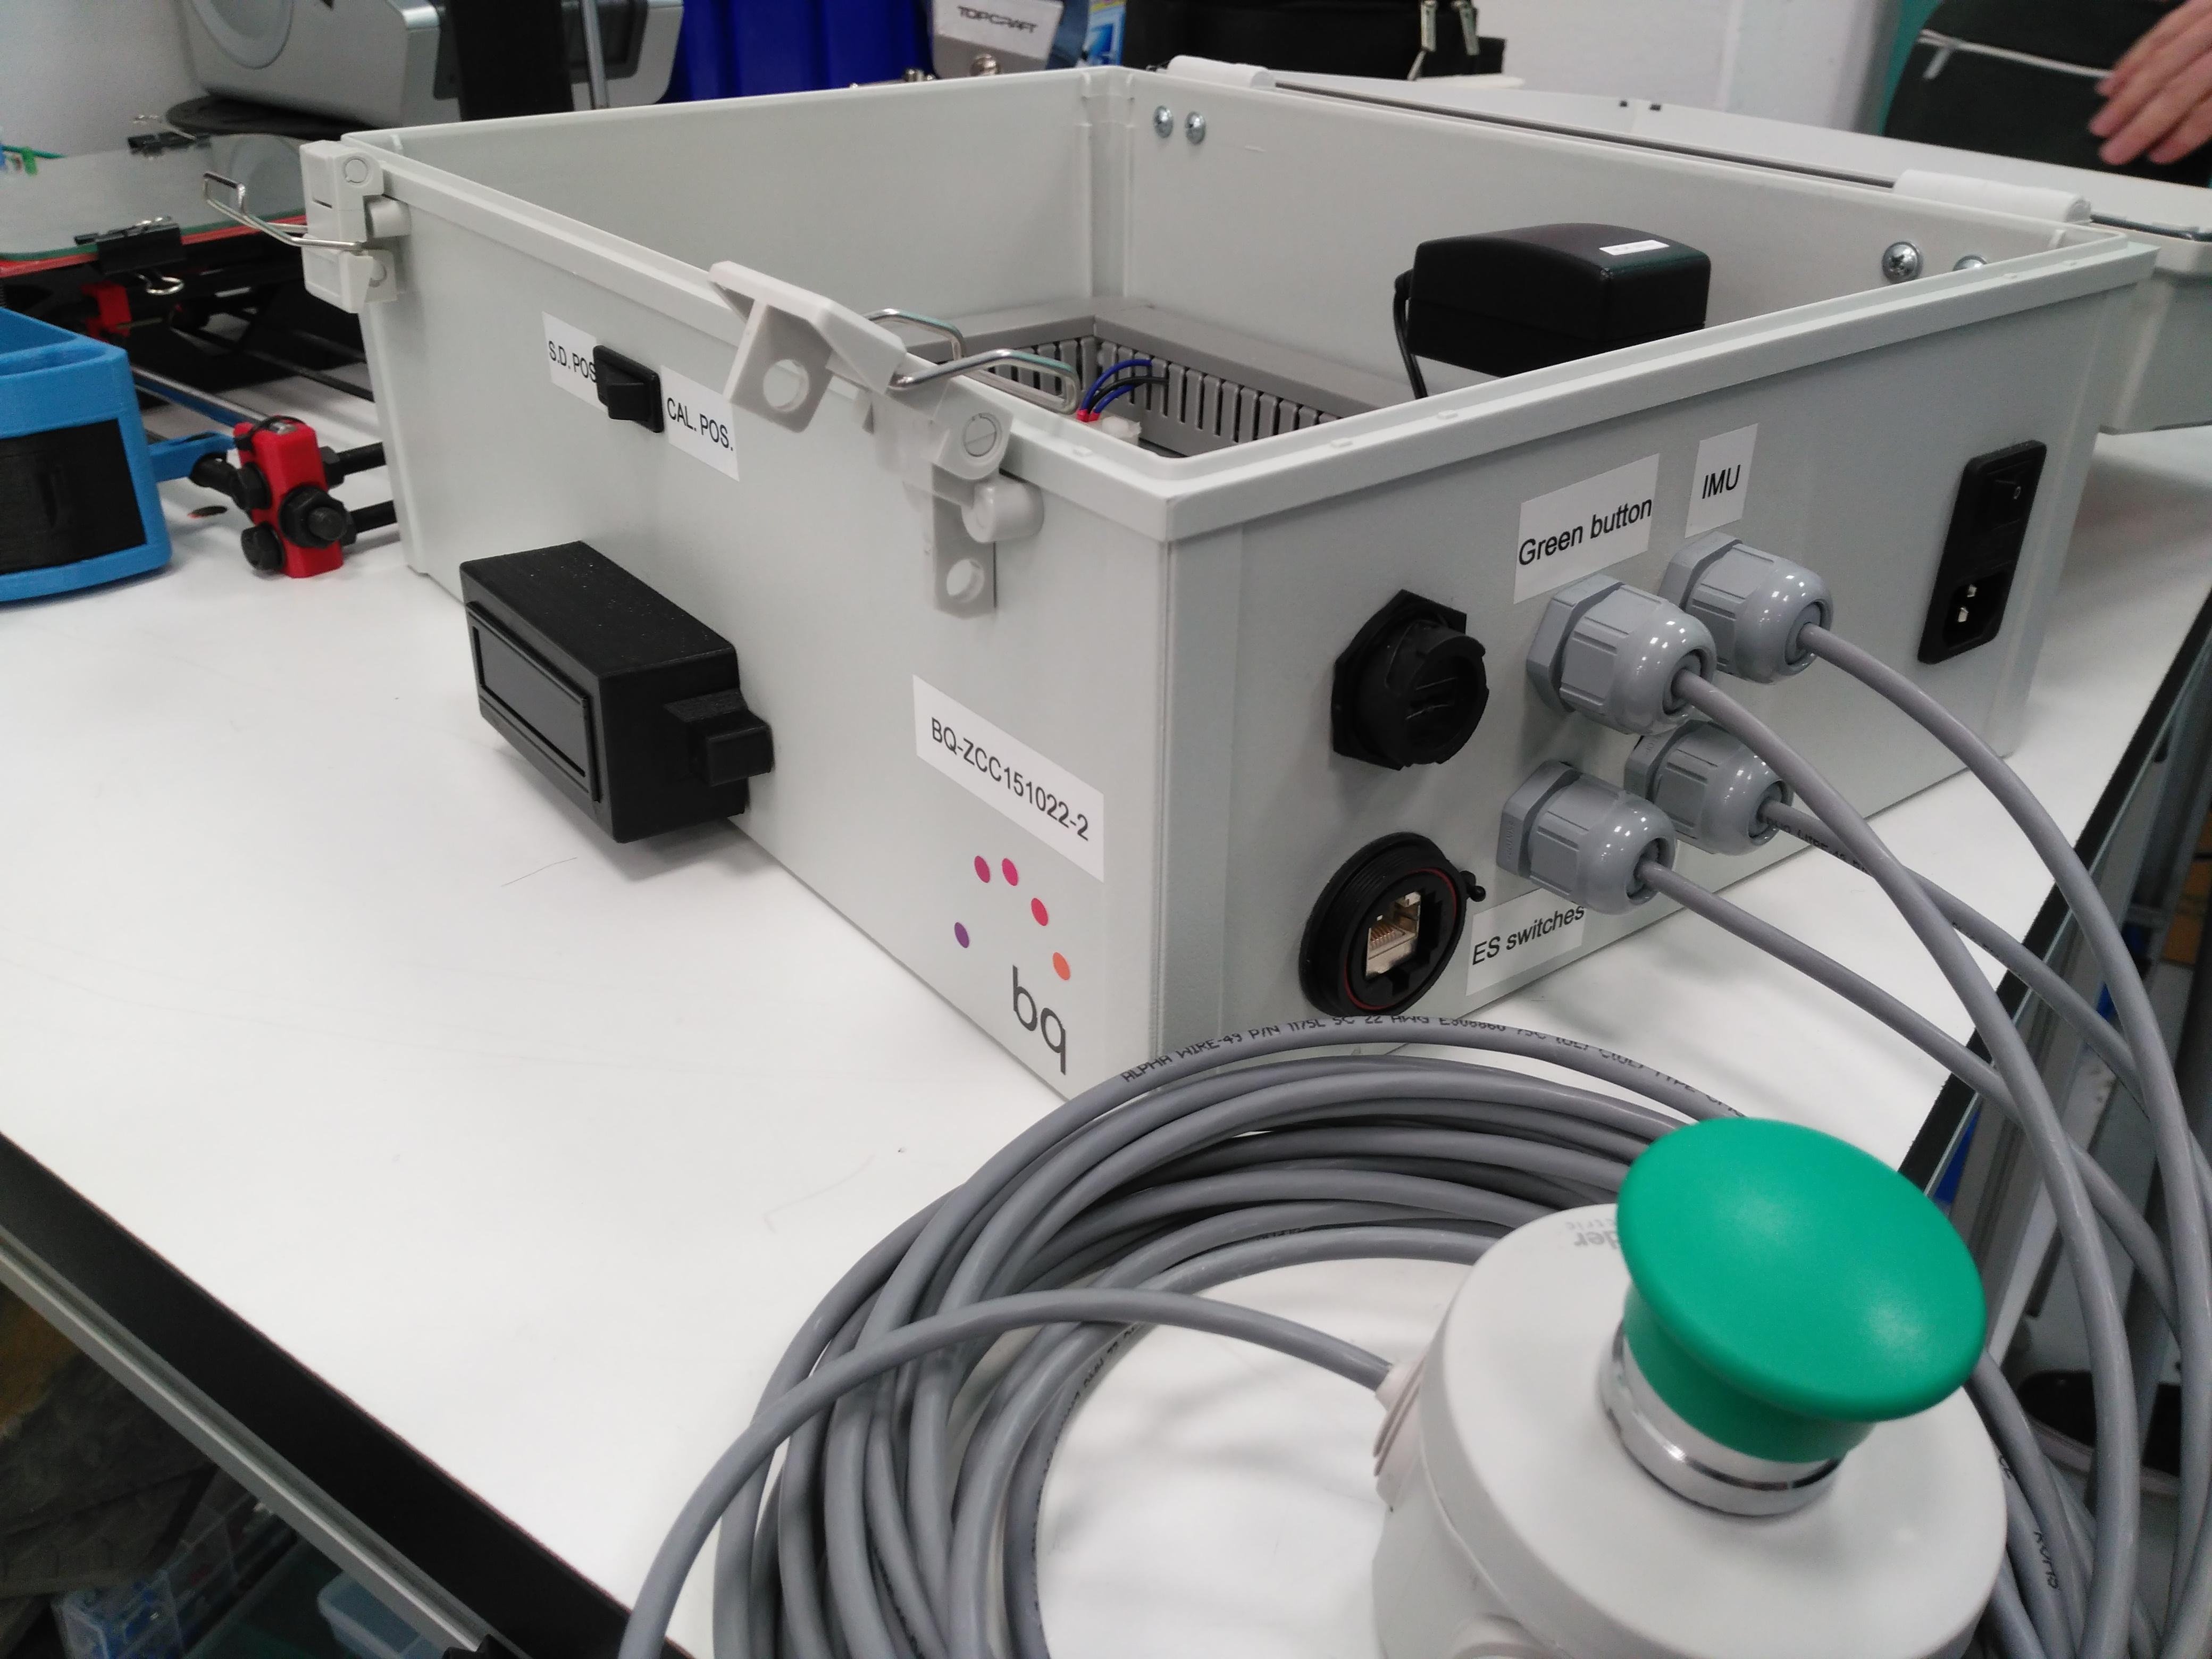
\includegraphics[width=120mm]{Figures/lateralArmario}
\caption{Armario final: Lateral}
\label{fig:lateralArmario}
\end{figure}

En el carril DIM se instala una toma de Schuko, al que se conectará la Raspberry PI para alimentar toda la electrónica. El armario es energizado por un conector a red eléctrica JR-101 con interruptor y fusible.

\begin{figure}
\centering
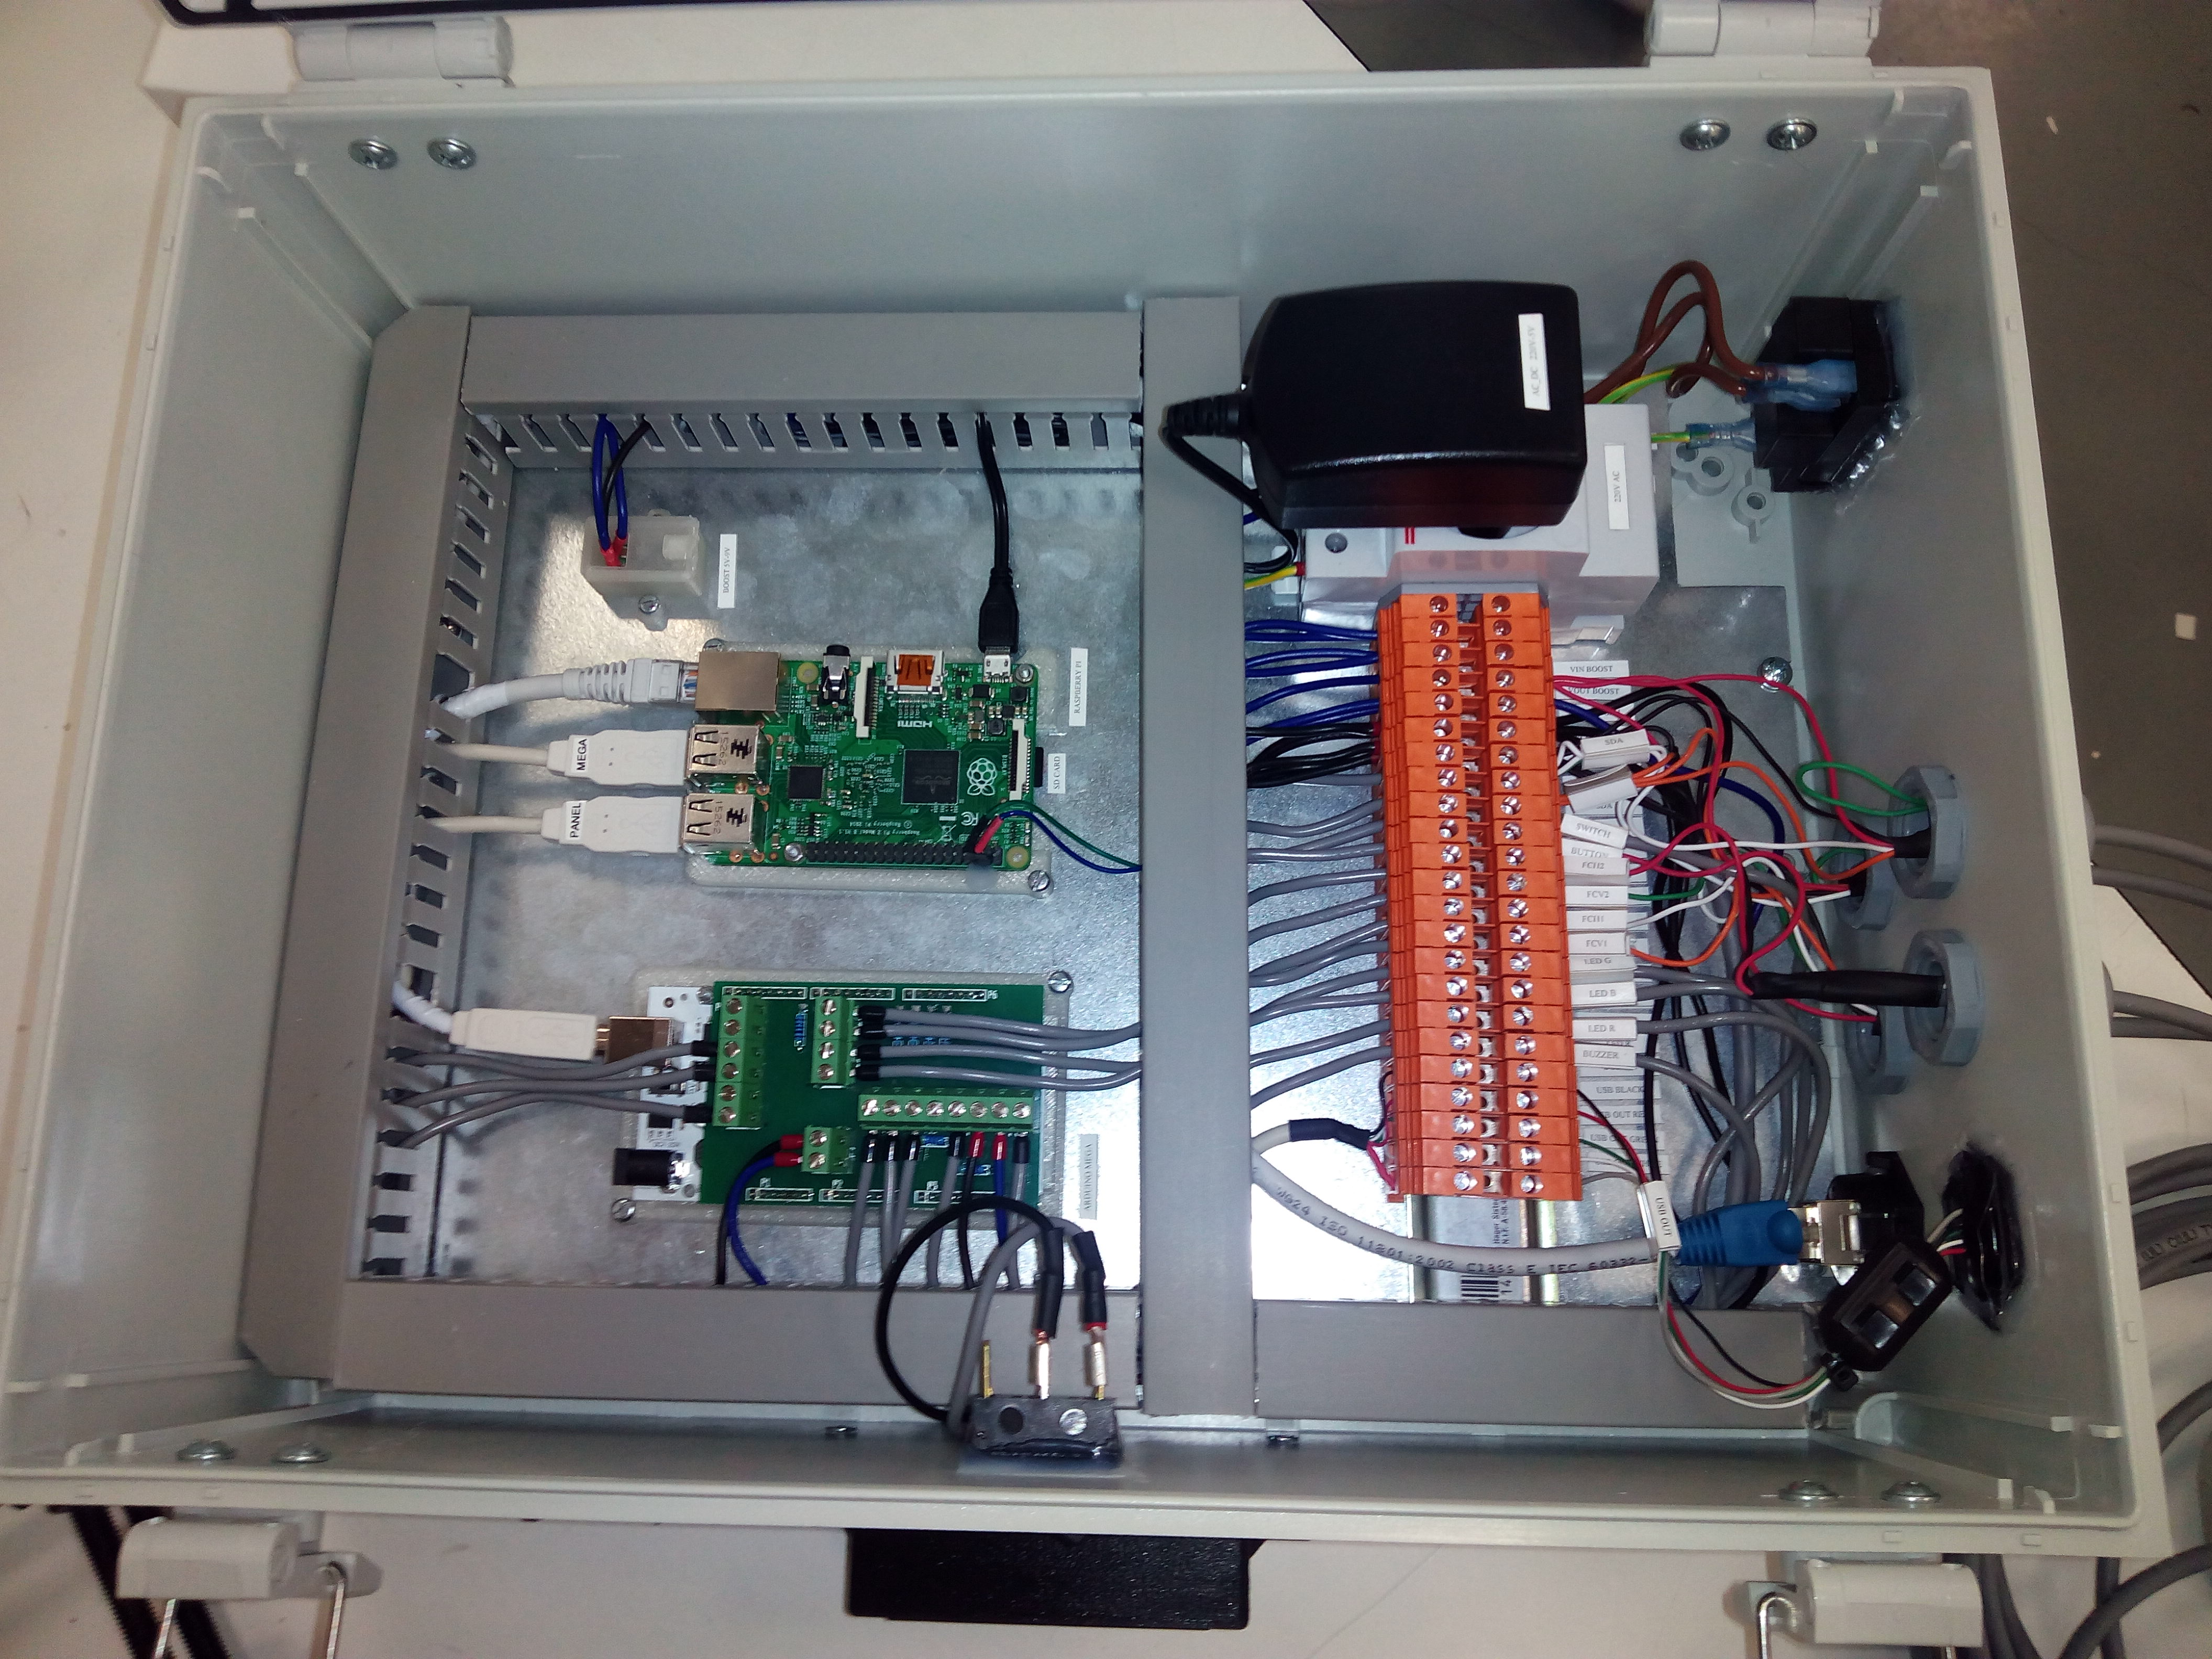
\includegraphics[width=120mm]{Figures/interiorArmario}
\caption{Armario final: Interior}
\label{fig:interiorArmario}
\end{figure}

Se pueden ver las Figuras \ref{fig:interiorArmario} y \ref{fig:lateralArmario}, interior y lateral del armario, respectivamente. Para detalle de las conexiones al clemero, se pueden consultar los planos eléctricos en el Anexo \ref{app:planosElectricos}.

\subsubsection{Mega}
Esta placa hace de cerebro del sistema a pesar de ser alimentada a través de la Raspberry, y de comunicar a través de ella con Zowi.

\begin{figure}
\centering
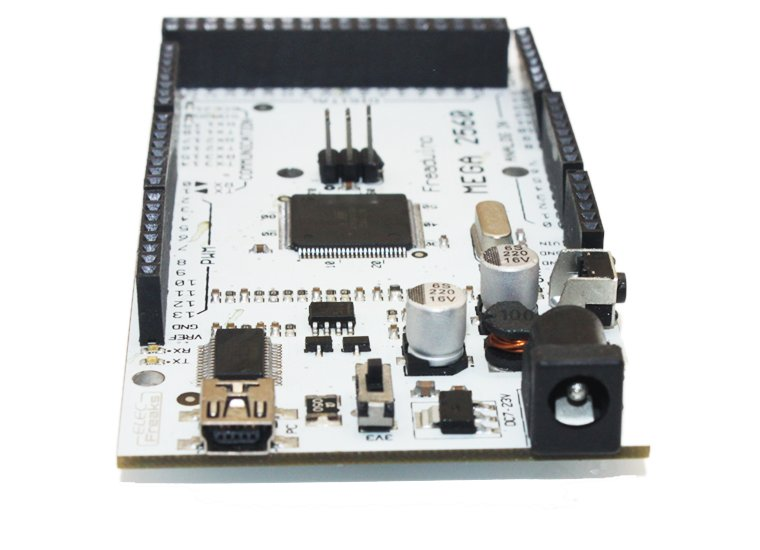
\includegraphics[width=90mm]{Figures/arduinoMega}
\caption{Mega}
\label{fig:arduinoMega}
\end{figure}

Recibe las lecturas de los sensores IMU, tiene conectados los finales de carrera, interruptor, pulsador, panel LCD, buzzer y leds. Todas las conexiones cableadas de entrada/salida, así como la alimentación pasan por un shield diseñado para ésta aplicación.

Define una máquina de estados que mueve al operador por todos los pasos de la calibración y controla a la raspberry mediante un protocolo de instrucciones implementado para este fin que usa como canal el puerto serie por USB, tambien empleado para hacer llegar instrucciones a la placa de Zowi.

Podemos decir que Mega es la encargada de interactuar con el exterior y, dentro de nuestro sistema, realiza las funciones de un PLC. Para ello se ha elegido cuidadosamente cómo conectar los diferentes componentes a sus entradas/salidas, en el Anexo \ref{app:pinoutMega} se puede consultar el pin-out de ésta placa:
\begin{itemize}
  \item Leds y buzzer necesitan PWM para poder configurar los sonidos/colores.
  \item Los pulsadores y finales de carrera se han conectado a entradas que tienen asociadas resistencias de pull-up, conectadas fácilmente por software.
  \item Se ha alimentado por Vin en lugar de por USB para poder alimentar a todos sus dispositivos.
\end{itemize}

Información sobre software en la Subsección \ref{subsec:Software}. Para conocer con detalle las conexiones se pueden consultar los documentos del Anexo \ref{app:PlanosElectricos}.

\subsubsection{Shield Mega}
Se emplea el diseño de la shield de la versión prototipo del armario. En este caso se mandan a fabricar las PCBs, ya que nuestra fresadora no dió unos resultados tan profesionales.

\begin{figure}
\centering
\begin{minipage}{.5\textwidth}
  \centering
  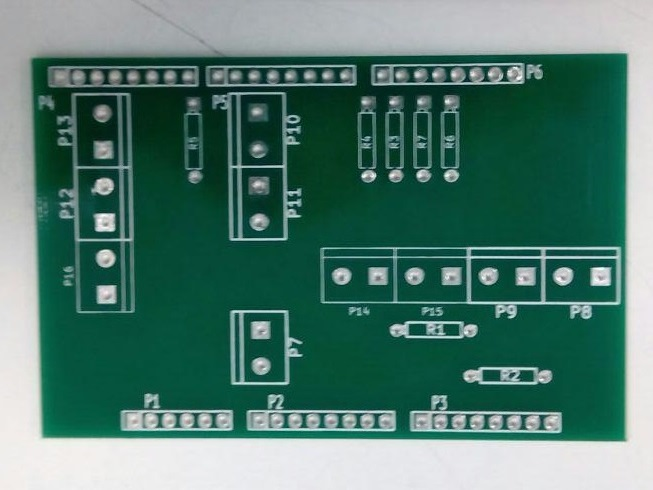
\includegraphics[width=.9\textwidth]{Figures/pcbMega}
  \captionof{figure}{Shield Mega soldada}
  \label{fig:pcbdMega}
\end{minipage}%
\begin{minipage}{.5\textwidth}
  \centering
  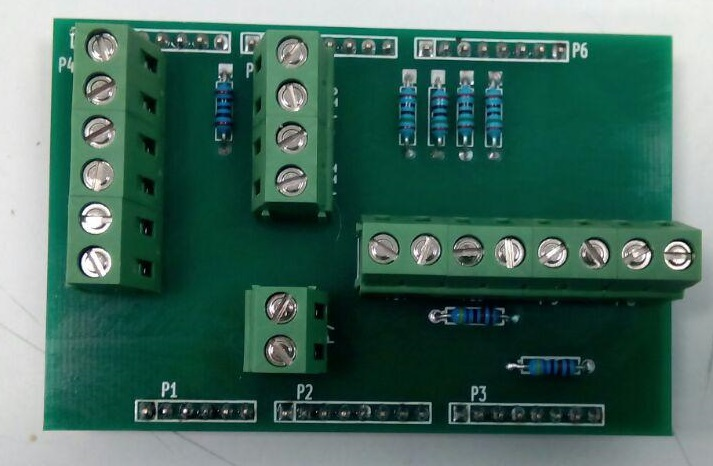
\includegraphics[width=.9\textwidth]{Figures/shieldMega}
  \captionof{figure}{PCB Shield Mega}
  \label{fig:shieldMega}
\end{minipage}
\end{figure}

Esta shield es colocada sobre los pines de la Mega y nos proporciona unos borneros para facilitar la conexión cableada a los dispositivos de entrada y salida, así como a la alimentación.

Los esquemáticos y gerbers con el layout del diseño de la PCB se pueden consultar en el Anexo \ref{app:pcbFiles}. Para información más clara sobre conexiones, se pueden consultar los planos eléctricos, en el Anexo \ref{app:planosElectricos}.

\subsubsection{Raspberry PI 2}

Este ordenador (Figura \ref{fig:raspi}) aporta muchísimas mejoras de fácil implementación al sistema, además de su función principal, hacer de enlace entre Mega y la controladora de Zowi. Éstas mejoras serán definidas en la Subsección \ref{subsec:Software}, apartado dedicado al software.

\begin{figure}
\centering
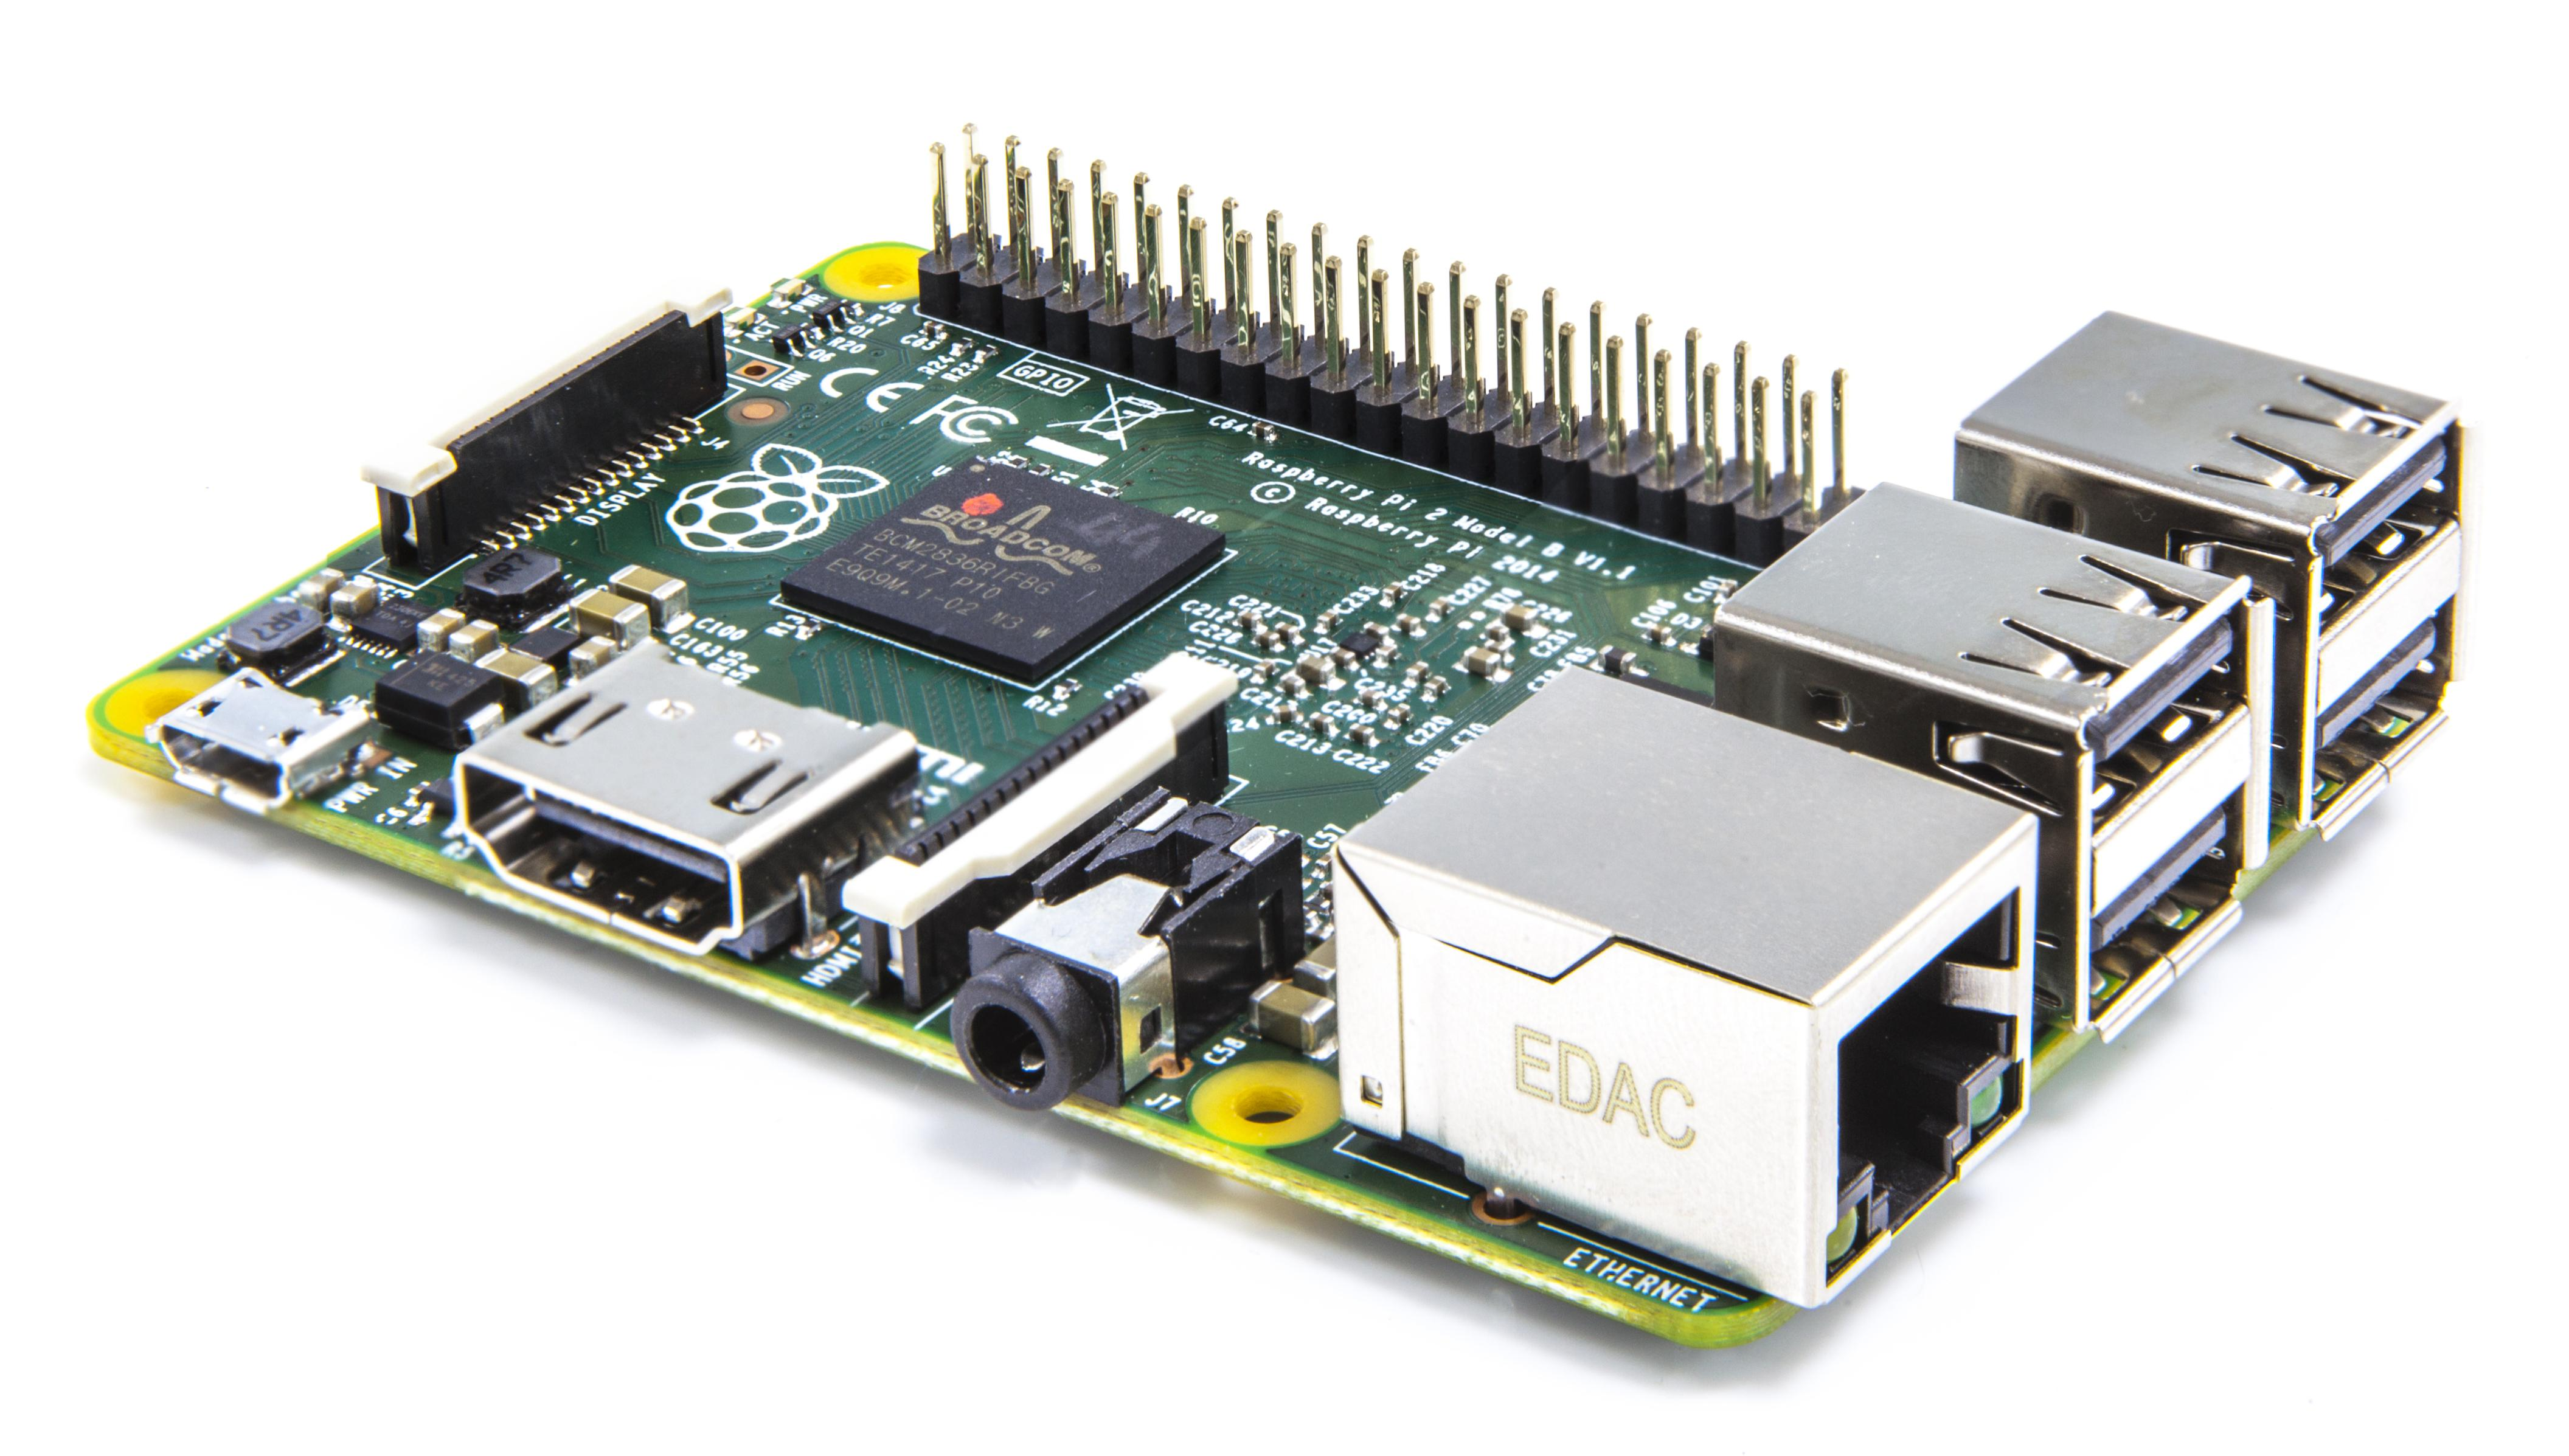
\includegraphics[width=100mm]{Figures/raspi}
\caption{Raspberry PI 2 - 1GB Ram}
\label{fig:raspi}
\end{figure}

Comunica con Mega y con las controladoras de los Zowi (Zum), para ello utiliza protocolo serie por cable USB con cada una de las placas. Además, por Ethernet, se puede acceder a ella por SSH (puerto 22) y por XRDP (puerto 3389) desde la misma red local o desde internet configurando propiamente el NAT; y una IP y puerto pueden ser configurados para guardar datos de calibración contra una base de datos remota.

Es alimentada por su toma microUSB, a través de un transformador conectado al Schuko del armario. Se encarga de alimentar y programar por USB a los Zowi, para lo que ha sido necesario desbloquear el límite de corriente suministrada por puerto USB por el sistema operativo (Se necesita suficiente potencia para mover los servos). También limenta a la Mega por su pin de 5V+, para lo que ha sido necesario elevar dicha tensión. Una vez más, se pueden ver los planos eléctricos para mayor detalle, Anexo \ref{planosElectricos}.

\subsubsection{Power Boost}

La Mega debe ser alimentada a más de 7V. Para reducir número de transformadores y el espacio ocupado, se decide alimentarla a través de la raspberry.

\begin{figure}
\centering
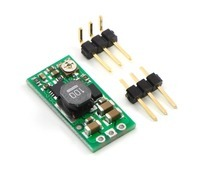
\includegraphics[width=70mm]{Figures/powerBoost}
\caption{Power Boost}
\label{fig:powerBoost}
\end{figure}

Este dispositivo (Figura \ref{fig:powerBoost}) acepta una tensión de entrada de 1.5V a 25V y, mediante el potenciómetro, permite ajustar su salida a valores entre 4V y 25V.

El power boost es ajustado para elevar la tensión suministrada por pines de la Raspberry de 5V a 9V para alimentar la Mega. Necesario para no tener que dar la corriente por el puerto USB. Aún desbloqueando el límite software de intensidad de la Raspberry, con lo que se consigue hasta 1.2A a 5V, el sistema no funciona correctamente al alimentar por USB ambas placas, Zowi carga su batería y mueve sus servos utilizando dicha corriente. De modo que se alimenta la Mega (y todo lo conectado a ella) desde el pin de 5v de Raspberry, sin usar el puerto USB y sin tener que introducir otro transformador en el armario.

\subsubsection{LCD Display}

Una pantalla es instalada para indicar al operador instrucciones e información sobre el uso del sistema. Se elige un display de 16 filas x 2 columnas y un backpack de Adafruit (Figura \ref{fig:backpack}) que nos permite comunicar con el display utilizando I\textsuperscript{2}C en lugar de una buena cantidad de salidas digitales, y que funciona con librerías más que probadas hechas por la comunidad.

\begin{figure}
\centering
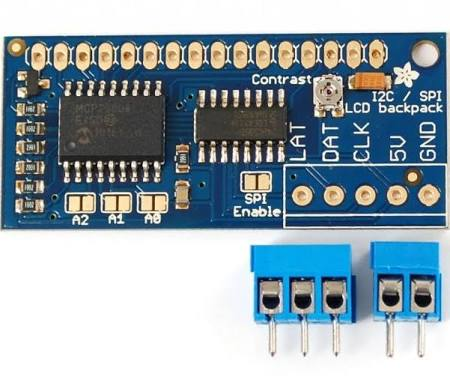
\includegraphics[width=75mm]{Figures/backpack}
\caption{Backpack para Display LCD}
\label{fig:backpack}
\end{figure}

\subsubsection{Otros componentes}

Además de los componentes principales comentados anteriormente, y de los sensores IMU tratados en el Marco Teórico (Capítulo \ref{ch:Chapter2}), se emplean otros componentes menores como son los leds, el buzzer, los botones, finales de carrera, así como sus resistencias, ademas de las clemas, puntas, y más. En los planos eléctricos (Anexo \ref{app:planosElectricos}) y hoja de costes (Anexo \ref{app:BOM}), se puede consultar más información sobre su conexión o modelo.

\subsubsection{Zowi - Zum}

Como se ha comentado anteriormente, Zowi también forma parte del sistema. Su controladora tendrá conectados, entre otras cosas, los 4 servomotores responsables de mover las articulaciones. Comunica solamente con la Raspberry PI utilizando protocolo serie por cable USB. La Raspberry le descargará un software para poder interpretar las instrucciones recibidas, y ser capaz de mover los servos o guardar información en su EEPROM.

\subsubsection{Banco soporte Final de Zowi y zapatos}

Para validaciones y durante todo el desarrollo del proyecto -así como para su uso en Madrid, tras acabar la fase de producción en fábrica- se han empleado, y emplean, los diseños realizados por el autor, cuyos planos podemos consultar en el Anexo \ref{app:planos}. No se especifican cotas de tolerancias por estar pensados para fabricar con impresoras 3D de filamento fundido, donde las dimensiones finales varían por parámetros como la temperatura o la velocidad de extrusión de la máquina.

\begin{figure}
\centering
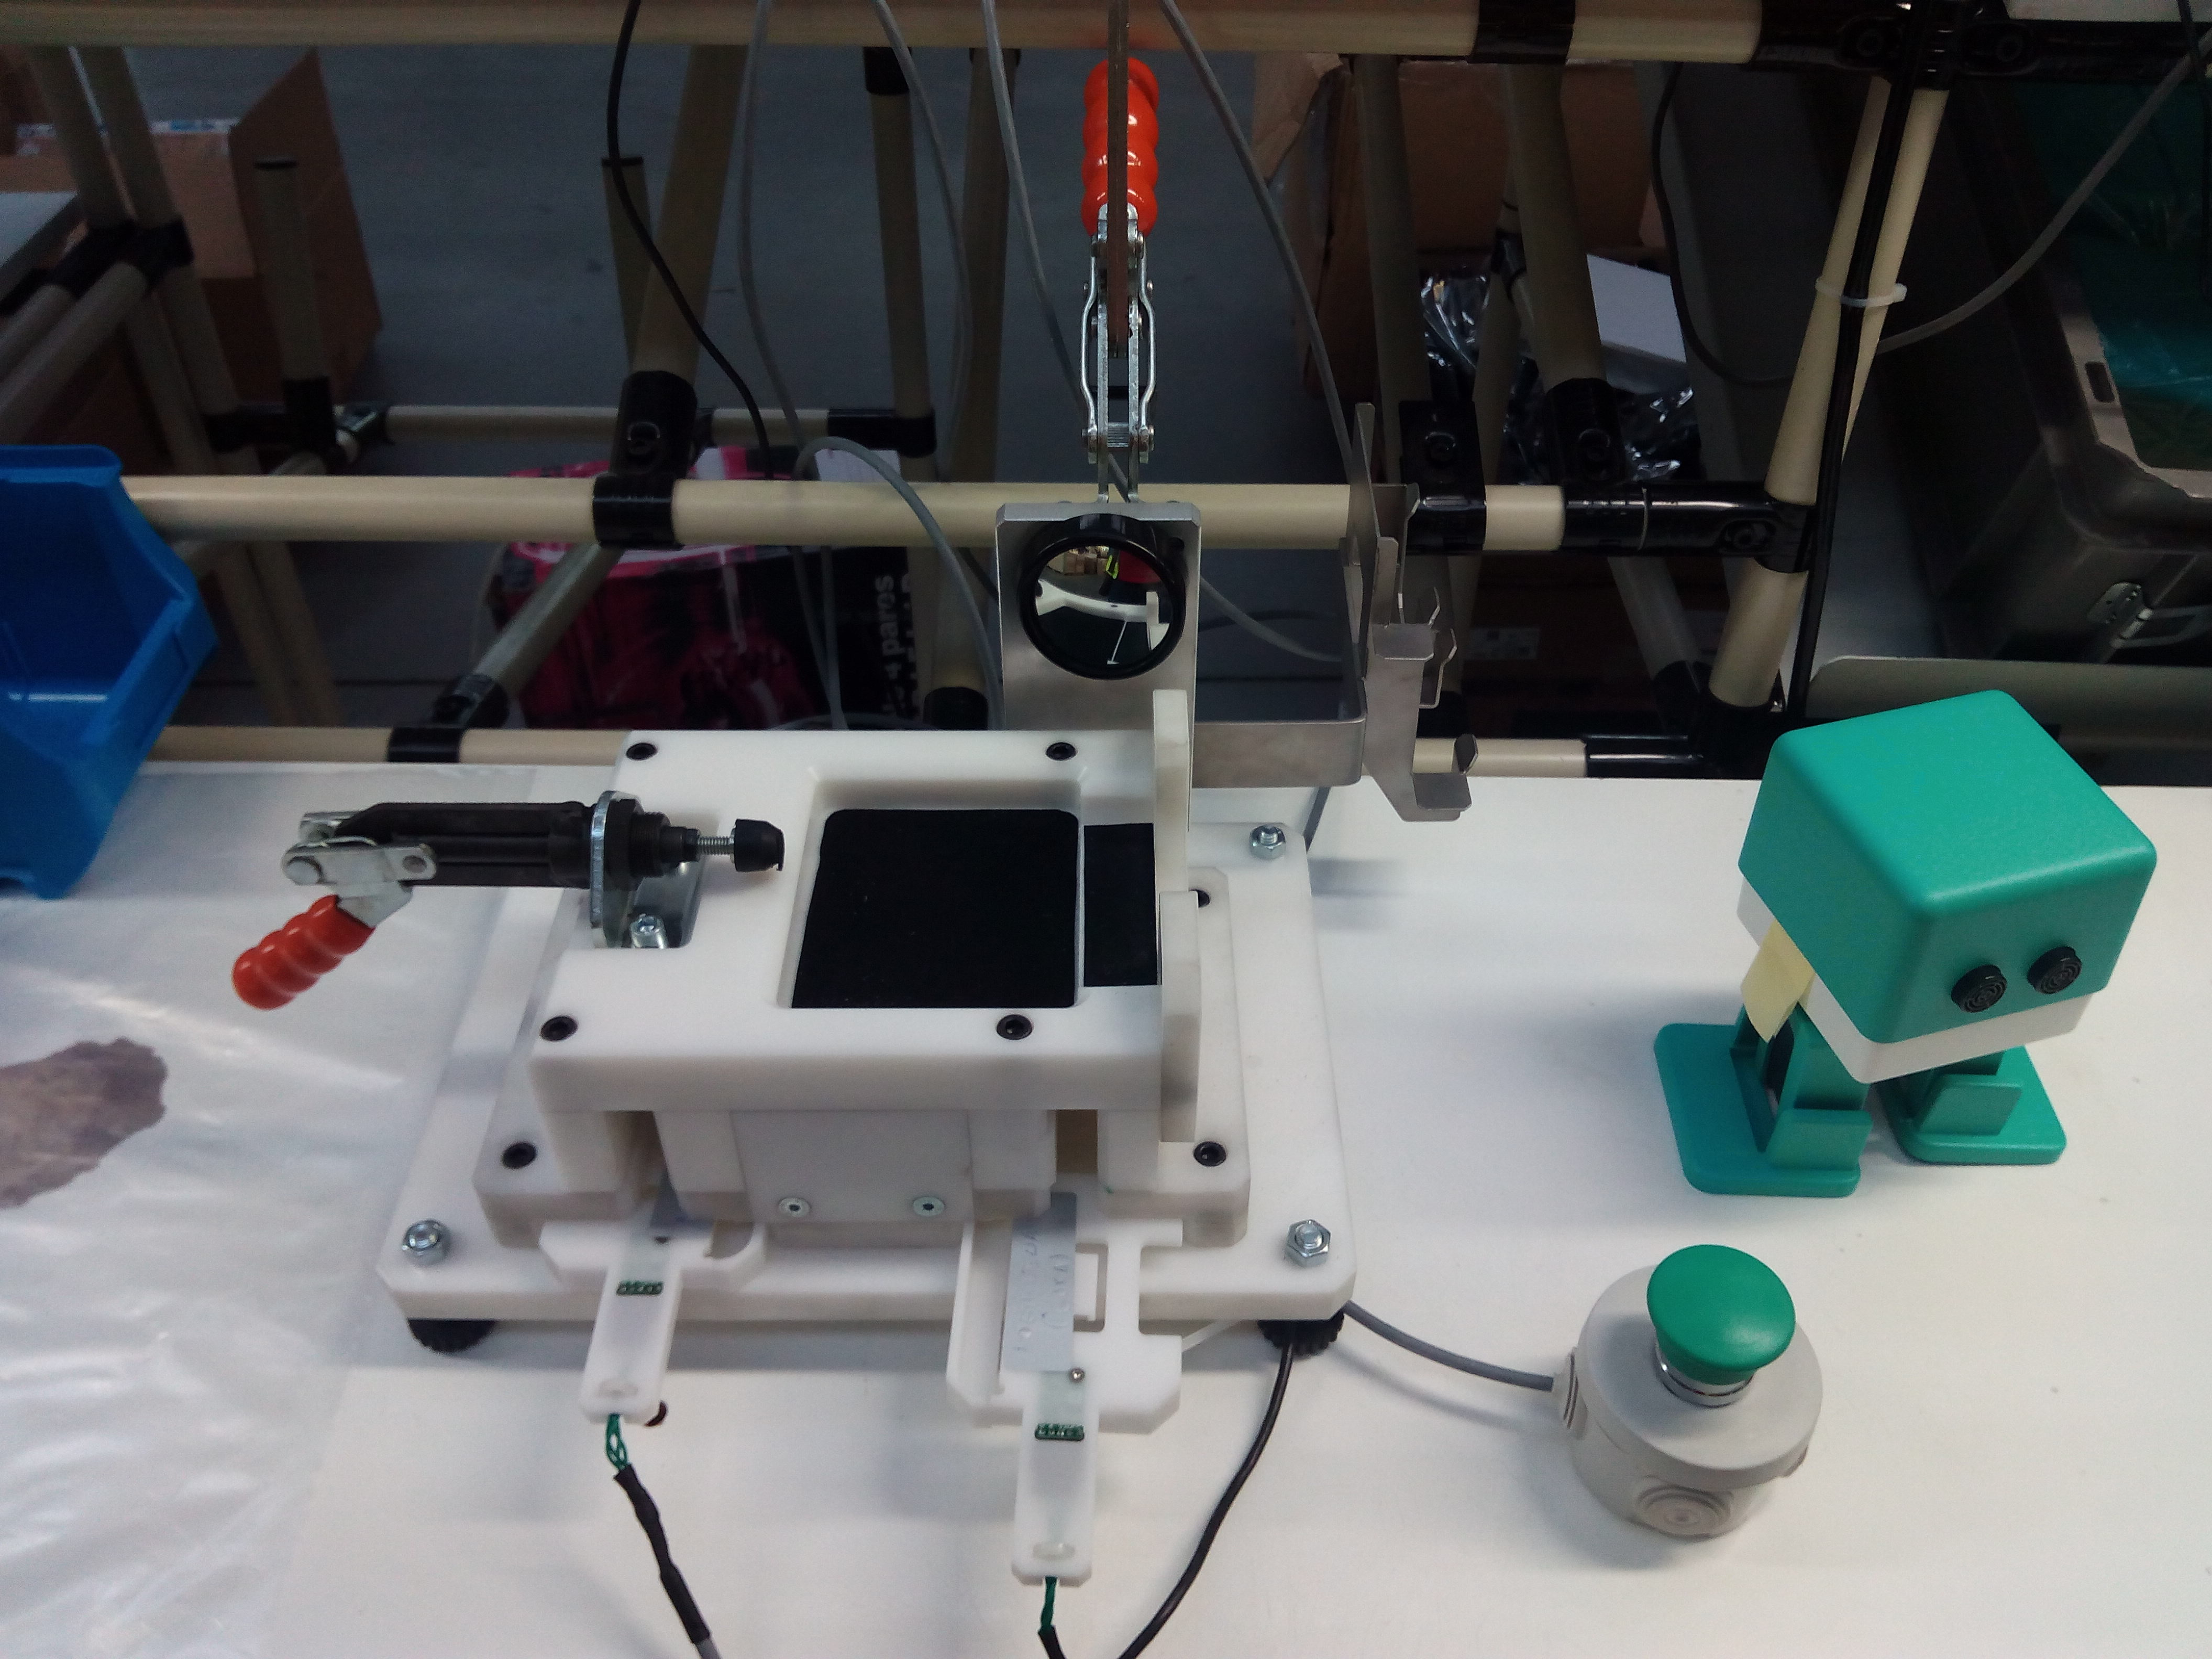
\includegraphics[width=120mm]{Figures/bancoFabrica}
\caption{Banco soporte y zapatos finales}
\label{fig:bancoFabrica}
\end{figure}

Sin embargo, el utillaje empleado en cadena de montaje (Figura \ref{fig:bancoFabrica}) fue rediseñado por el Dpto. de Mecánica y fabricado por sinterizado selectivo por láser, para lograr un acabado más preciso y mayor resistencia. Le añadieron palancas para fijar cada juguete y mejoraron los zapatos para facilitar la colocación.

%-----------------------------------
%	SUBSECTION 2
%-----------------------------------

\subsection{Software}
\label{subsec:Software}

Subsección en desarrollo. (Estimado 6-7 páginas sin fotos con alguans tablas.)

Intérprete - comunicacion entre las placas. Tabla comandos serie.

Programa, máquina estados, librerías Mega -> Anexo diagramas, codigos.

Raspberry, python, demon/autoarranque -> Anexo software, scripts linux.

Perks: SQL, Arduino Suite, escritorio remoto -> Anexo how-tos¿?, estructura SQL

Fixes: Detección placa conectada -> Off/On del puerto USB para debug.
